\chapter{Selective Prediction via Training Dynamics}

% \section{Additional Related Selective Prediction Works}

%  Additional related approaches we highlight beyond Section~\ref{ssec:related}: performing statistical inference for the marginal prediction-set coverage rates using model ensembles~\citep{feng2021selective}, confidence prediction using an earlier snapshot of the model~\citep{geifman2018bias}, estimating the gap between classification regions corresponding to each class~\citep{gangrade2021selective}, and complete precision by classifying only when models consistent with the training data predict the same output~\citep{khani2016unanimous}. 

% \section{Extended Discussion on Example Difficulty}
% \label{sec:example_diff}

% A related line of work is identifying \emph{difficult} examples, or how well a model can generalize to a given unseen example. 
% \citet{jiang2020characterizing} introduce a per-instance empirical consistency score which estimates the probability of predicting the ground truth label with models trained on data subsamples of different sizes. Unlike our approach, however, this requires training a large number of models. 
% ~\citet{toneva2018empirical} quantifies example difficulty through the lens of a forgetting event, in which the example is misclassified after being correctly classified. However, the metrics that we introduce in \S~\ref{sec:method}, are based on the disagreement of the label at each checkpoint with the final predicted label. Other approaches estimate the example difficulty by: 
% prediction depth of the first layer at which a $k$-NN classifier correctly classifies an example~\citep{baldock2021deep}, the impact of pruning on model predictions of the example~\citep{hooker2019compressed}, and estimating the leave-one-out influence of each training example on the accuracy of an algorithm by using influence functions~\citep{feldman2020neural}. 
% Closest to our method, the work of \citet{agarwal2020estimating} utilizes gradients of intermediate models during training to rank examples by  difficulty. In particular, they average pixel-wise variance of gradients for each given input image. 
% Notably, this approach is more costly and less practical than our approach and also does not study the accuracy/coverage trade-off which is of paramount importance to selective prediction.



\section{Alternate Metric Choices}
\label{sec:alt_scores}

We briefly discuss additional potential metric choices that we investigated but which lead to selective classification performance worse than our main method.

% \subsection{Incorporating Estimates of $e_t$ into \smin and \savg} Since the results in  \S~\ref{ssec:ver_ei_vi} show that $e_t$ is only nearly $0$ almost everywhere, we investigate whether incorporating an estimate of $e_t$ into \smin and \savg leads to additional SC improvements. Our results demonstrate that neither an empirical estimate nor a smooth decay function similar to $v_t$ robustly improves over \smin and \savg (which assumed $e_t = 0$).

\subsection{Jump Score \sjmp} We also consider a score which captures the level of disagreement between the predicted label of two successive intermediate models (\ie how much jumping occurred over the course of training). For $j_t = 0$ iff $f_{t}(\bm{x}) = f_{t-1}(\bm{x})$ and $j_t = 1$ otherwise we can compute the jump score as $s_\text{jmp} = 1 - \sum v_t j_t$ and threshold it as in \S~\ref{ssec:min_score} and \S~\ref{ssec:avg_score}. 

\subsection{Variance Score \svar for Continuous Metrics}

\begin{contriback}
This subsection was written with Kimia Hamidieh.
\end{contriback}

We consider monitoring the evolution of continuous metrics that have been shown to be correlated with example difficulty. These metrics include (but are not limited to):
\begin{itemize}
	\item Confidence (conf): $\max _{c \in \mathcal{Y}} f_{t}(\bm{x})$
	\item Confidence gap between top 2 most confident classes (gap): $\max _{c \in \mathcal{Y}} f_{t}(\bm{x})  - \max _{c \not = \hat{y}} f_{t}(\bm{x})$
	\item Entropy (ent): $-\sum_{c=1}^C f_{t}(\bm{x})_c \log \left(f_{t}(\bm{x})_c\right)$
\end{itemize}
\cite{jiang2020characterizing} show that  
example difficulty is correlated with confidence and entropy. Moreover, they find that difficult examples are learned later in the training process. This observation motivates designing a score based on these continuous metrics that penalises changes later in the training process more heavily.
We consider the maximum softmax class probability known as confidence, the negative entropy and the gap between the most confident classes for each example instead of the model predictions. 
Assume that any of these metrics is given by a sequence $z = \{z_1,\ldots,z_T\}$ obtained from $T$ intermediate models. Then we can capture the uniformity of $z$ via a (weighted) variance score $s_\text{var} = \sum_{t} w_t (z_t - \mu)^2$ for mean $\mu = \frac{1}{T}\sum_{t} z_t$ and an increasing weighting sequence $w = \{w_1,\ldots,w_T\}$.

In order to show the effectiveness of the variance score \svar for continuous metrics, we provide a simple bound on the variance of confidence  $\max _{y \in \mathcal{Y}} f_{t}(\bm{x})$ in the final checkpoints of the training. 
Assuming that the model has converged to a local minima with a low learning rate, we can assume that the distribution of model weights can be approximated by a Gaussian distribution. 

We consider a linear regression problem where the inputs are linearly separable. 

\begin{lemma}
Assume that we have some Gaussian prior on the model parameters in the logistic regression setting across $m$ final checkpoints. More specifically, given $T$ total checkpoints of model parameters $\{\bm{w}_1, \bm{w_2}, \dots, \bm{w}_T \}$ we have $p(W = \bm{w}_t) = \mathcal{N}(\bm{w}_0 \mid \bm{\mu}, s\bm{I}) $ for $t \in \{T - m + 1, \dots, T\}$ and we assume that final checkpoints of the model are sampled from this distribution. We show that the variance of model confidence $ \max_{y \in \{-1, 1\}} p(y \mid \bm{x}_i, \bm{w}_t)$ for a datapoint $(\bm{x}_i, y_i)$ can be upper bounded by a factor of probability of correctly classifying this example by the optimal weights. 

\end{lemma}

\begin{proof}
We first compute the variance of model predictions $p(y_i \mid \bm{x}_i, W)$ for a given datapoint $(\bm{x}_i, y_i)$. Following previous work~\citep{schein2007active, chang2017active}, the variance of predictions over these checkpoints can be estimated as follows:

Taking two terms in Taylor expansion for model predictions we have $p(y_i \mid \bm{x}_i, W) \simeq p(y_i \mid \bm{x}_i, \bm{w}) + g_i(\bm{w})^\top (W - \bm{w})$ where $W$ and $\bm{w}$ are current and the expected estimate of the parameters and $g_i(\bm{w}) = p(y_i \mid \bm{x}_i, \bm{w}) (1 - p(y_i \mid \bm{x}_i, \bm{w}))\bm{x}_i $ is the gradient vector. Now we can write the variance with respect to the model prior as: 
$$ \mathbb{V}\left( p(y_i \mid \bm{x}_i, W) \right ) \simeq \mathbb{V}\left( g_i(\bm{w})^\top (W - \bm{w}) \right ) =  g_i(\bm{w})^\top F^{-1}  g_i(\bm{w})$$ where $F$ is the variance of posterior distribution $p(W \mid X, Y) \sim \mathcal{N}(W \mid \bm{w}, F^{-1})$. 
This suggests that the variance of probability of correctly classifying $\bm{x}_i$ is proportional to $p(y_i \mid \bm{x}_i, \bm{w})^2 (1 - p(y_i \mid \bm{x}_i, \bm{w}))^2$. Now we can bound the variance of maximum class probability or confidence as below:
\begin{align*}
  \mathbb{V}\left( \max_{y \in \{-1, 1\}} p(y \mid \bm{x}_i, W) \right ) & \leq  \mathbb{V}\left( p(y_i \mid \bm{x}_i, W) \right ) +  \mathbb{V}\left( p(- y_i \mid \bm{x}_i, W) \right ) \\
  & \approx 2 p(y_i \mid \bm{x}_i, \bm{w})^2 (1 - p(y_i \mid \bm{x}_i, \bm{w}))^2 \bm{x}_i^\top F^{-1} \bm{x}_i 
\end{align*}
\end{proof}
We showed that if the probability of correctly classifying an example given the final estimate of model parameters is close to one, the variance of model predictions following a Gaussian prior gets close to zero, we expect a similar behaviour for the variance of confidence under samples of this distribution. 

\section{Extension of Empirical Evaluation}

\subsection{Full Hyper-Parameters }
\label{app:baseline_hyperparams}

We document full hyper-parameter settings for our method (\sptd) as well as all baseline approaches in Table~\ref{tab:hyperpar}.

\begin{table*}[ht]
    \centering 
        \caption[Hyper-parameters used for all algorithms for classification.]{\textbf{Hyper-parameters used for all algorithms for classification.}}
    \label{tab:hyperpar}
     \begin{tabular}{@{}c c c@{}} 
     \toprule
     Dataset & SC Algorithm & Hyper-Parameters \\ 
     \midrule
     \multirow{4}{*}{CIFAR-10}      & Softmax Response (\sr) & N/A \\ 
                      & Self-Adaptive Training (\sat)  & $P=100$\\ 
                      & Deep Ensembles (\de)  & $E=10$\\ 
                      & Selective Prediction Training Dynamics (\sptd) & $T = 1600,\ k=2$ \\ 
     \midrule
     \multirow{4}{*}{CIFAR-100}      & Softmax Response (\sr) & N/A \\ 
                      & Self-Adaptive Training (\sat)  & $P=100$\\ 
                      & Deep Ensembles (\de)  & $E=10$\\ 
                      & Selective Prediction Training Dynamics (\sptd) & $T = 1600,\ k=2$ \\ 
     \midrule
     \multirow{4}{*}{Food101}      & Softmax Response (\sr) & N/A \\ 
                      & Self-Adaptive Training (\sat)  & $P=100$\\ 
                      & Deep Ensembles (\de)  & $E=10$\\ 
                      & Selective Prediction Training Dynamics (\sptd) & $T = 2200,\ k=3$ \\
    \midrule
    \multirow{4}{*}{StanfordCars}      & Softmax Response (\sr) & N/A \\ 
                      & Self-Adaptive Training (\sat)  & $P=100$\\ 
                      & Deep Ensembles (\de)  & $E=10$\\ 
                      & Selective Prediction Training Dynamics (\sptd) & $T = 800,\ k=5$ \\
     \bottomrule
    \end{tabular}
\end{table*}

\subsection{Additional Selective Prediction Results}
\label{app:add_exp}

% \subsubsection{Variance Score Experiments on Continuous Metrics} In addition to the evolution of predictions made across intermediate models, we also monitor a variety of easily computable continuous metrics. In our work, we consider the following metrics:
% \begin{itemize}
% 	\item Confidence (conf): $\max _{c \in \mathcal{Y}} f_{t}(\bm{x})$
% 	\item Confidence gap between top 2 most confident classes (gap): $\max _{c \in \mathcal{Y}} f_{t}(\bm{x})  - \max _{c \not = \hat{y}} f_{t}(\bm{x})$
% 	\item Entropy (ent): $-\sum_{c=1}^C f_{t}(\bm{x})_c \log \left(f_{t}(\bm{x})_c\right)$
% \end{itemize}
% Note that for the purpose of this experiment, we adapt the notation of $f$ to map to a softmax-parameterized output instead of the hard thresholded label, formally $f: \mathcal{X} \rightarrow \mathbb{R}^{|\mathcal{Y}|}$. 

% We depict example evolution plots for these metrics in Figures~\ref{fig:svhn_ext}, \ref{fig:gtsrb}, \ref{fig:cifar10}, \ref{fig:cifar100}, and \ref{fig:catsdogs} in the third row.

% \subsubsection{Individual Metric Evolution Plots} We provide additional individual metric evolution plots for SVHN (Figure~\ref{fig:svhn_ext}), GTSRB (Figure~\ref{fig:gtsrb}), CIFAR-10 (Figure~\ref{fig:cifar10}), CIFAR-100 (Figure~\ref{fig:cifar100}), and Cats \& Dogs (Figure~\ref{fig:catsdogs}).

\subsubsection{Extended Synthetic Experiments}

We extend the experiment from Figure~\ref{fig:gauss} to all tested SC methods in Figure~\ref{fig:gauss_ext}. We also provide an extended result using Bayesian Linear Regression in Figure~\ref{fig:blr}.

\begin{figure*}[t]
  \centering
  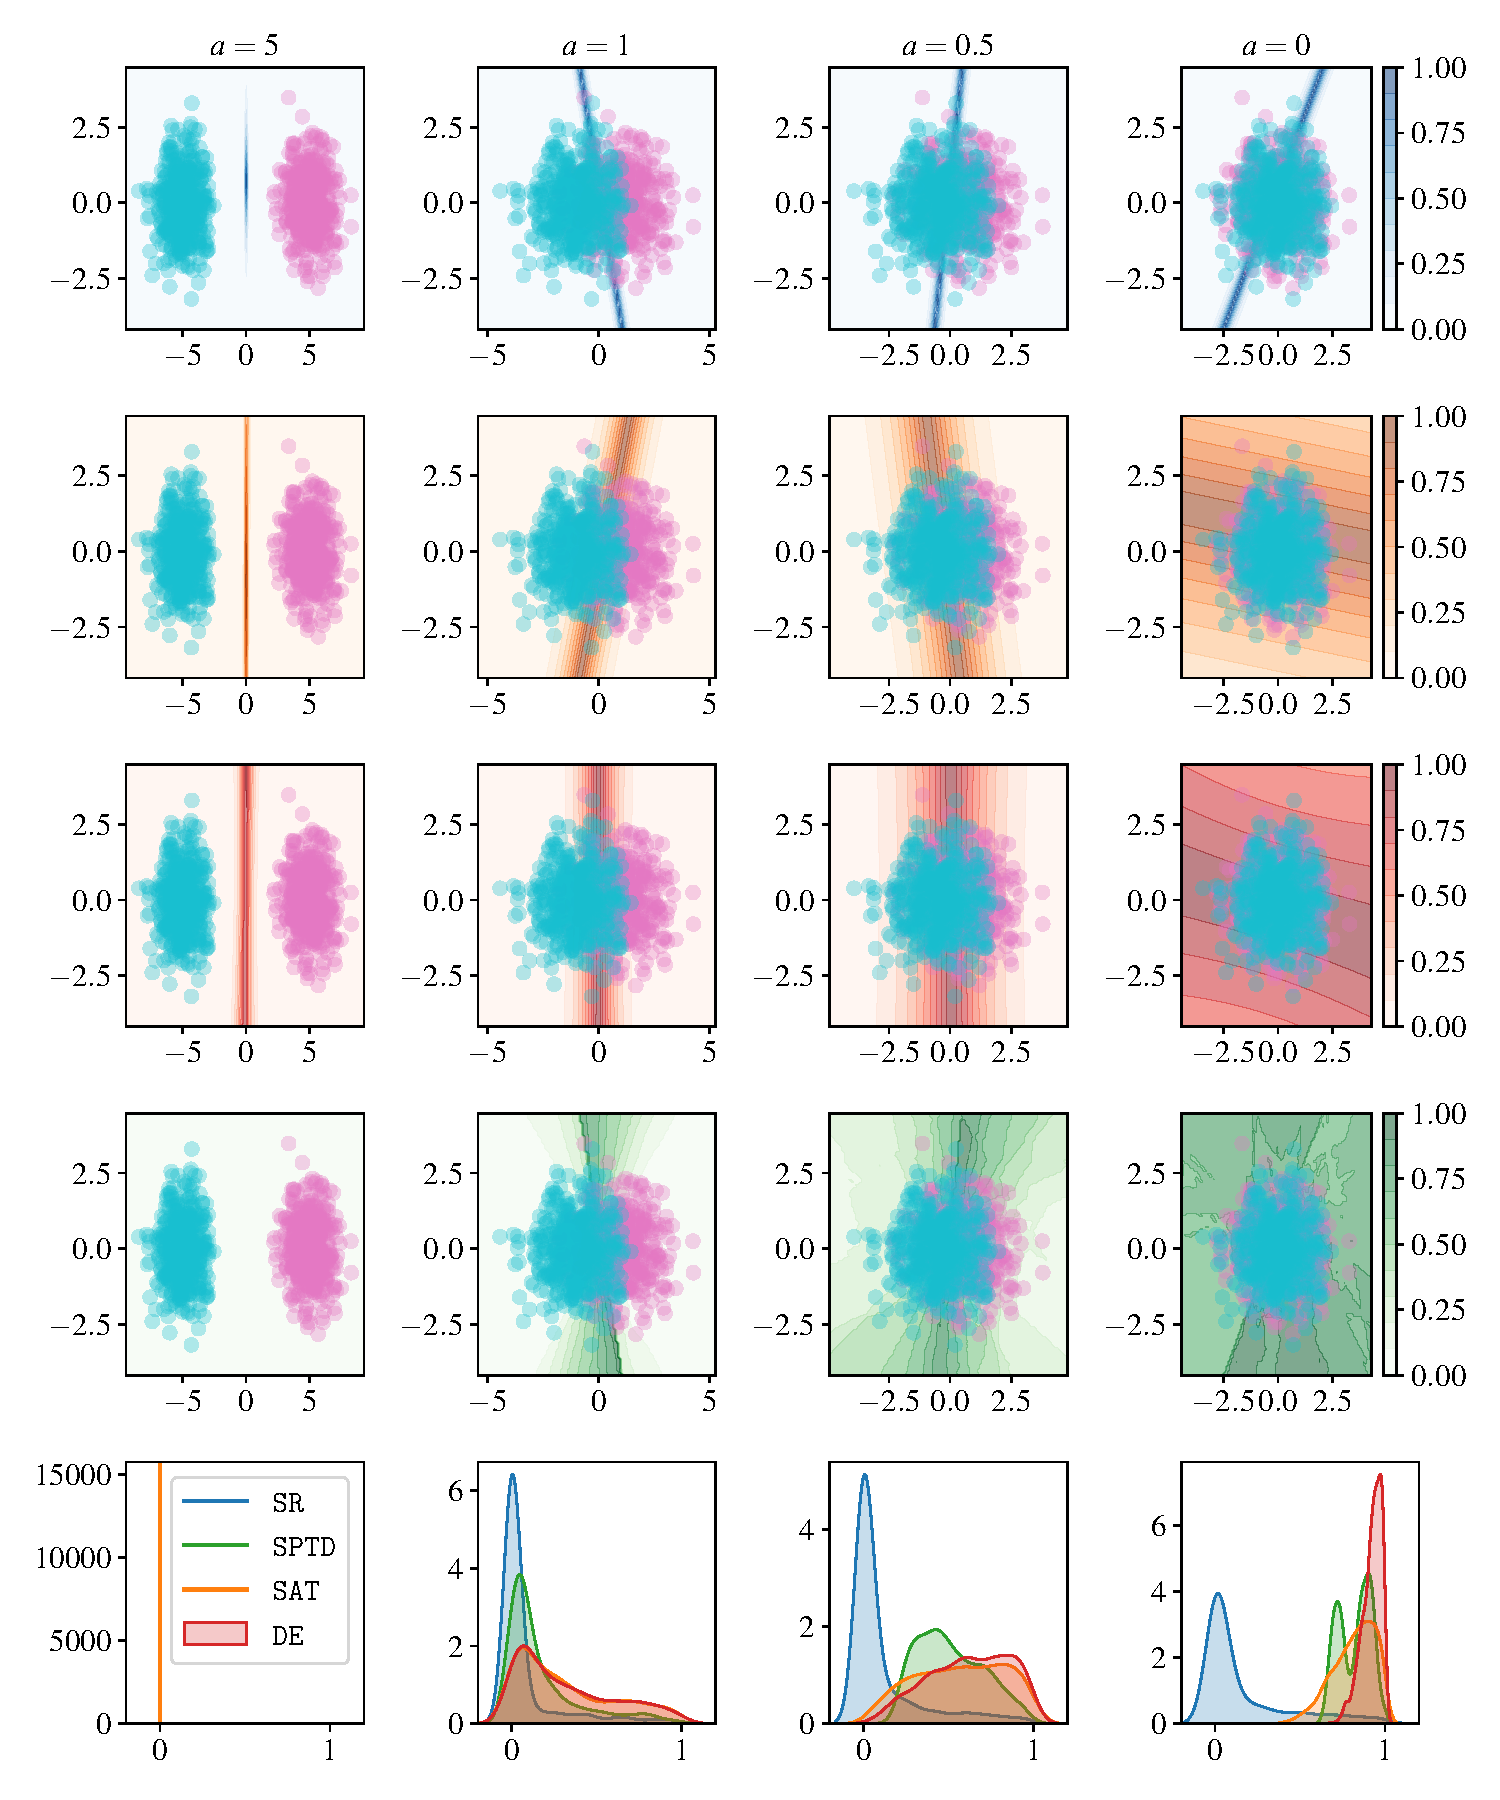
\includegraphics[width=0.95\linewidth]{figs/sptd/gaussians_2.pdf}
\caption[Extended Gaussian experiment.]{\textbf{Extended Gaussian experiment.}  The first row corresponds to the anomaly scoring result of \sr, the second to the result of \sat, the third to the result of \de, and the fourth to the result of \sptd. The bottom row shows the score distribution for each method over the data points. We see that all methods reliably improve over the \sr baseline. At the same time, we notice that \sat and \de still assign higher confidence away from the data due to limited use of decision boundary oscillations. \sptd addresses this limitation and assigns more uniform uncertainty over the full data space.}
\label{fig:gauss_ext}
\end{figure*}

\begin{figure*}[t]
  \centering
  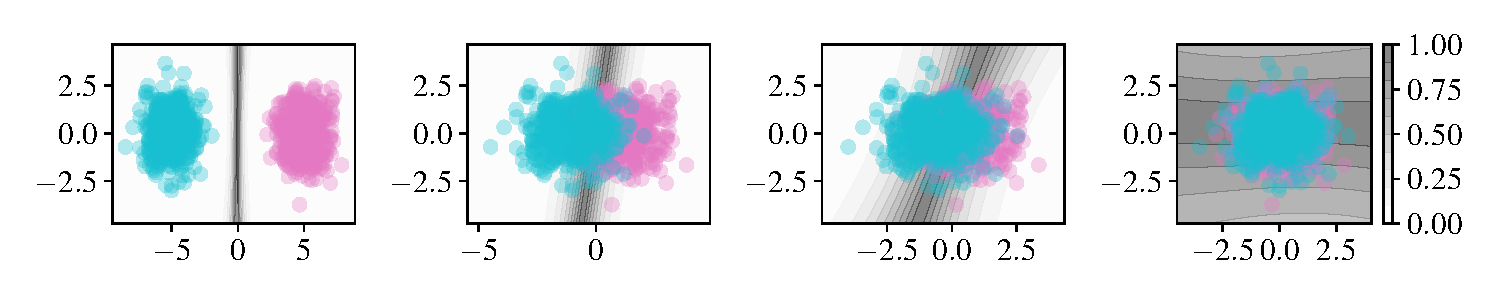
\includegraphics[width=\linewidth]{figs/sptd/blr.pdf}
\caption[Bayesian linear regression experiment on Gaussian data.]{\textbf{Bayesian linear regression experiment on Gaussian data.} Results comparable to \de.}
\label{fig:blr}
\end{figure*}

% \newlyadded{
% \subsubsection{Full Score Distribution}

% We extend the experiment from Figure~\ref{fig:scores} to all tested SC methods in Figure~\ref{fig:scores_ext}.

% \begin{figure*}[t]
%   \centering
%   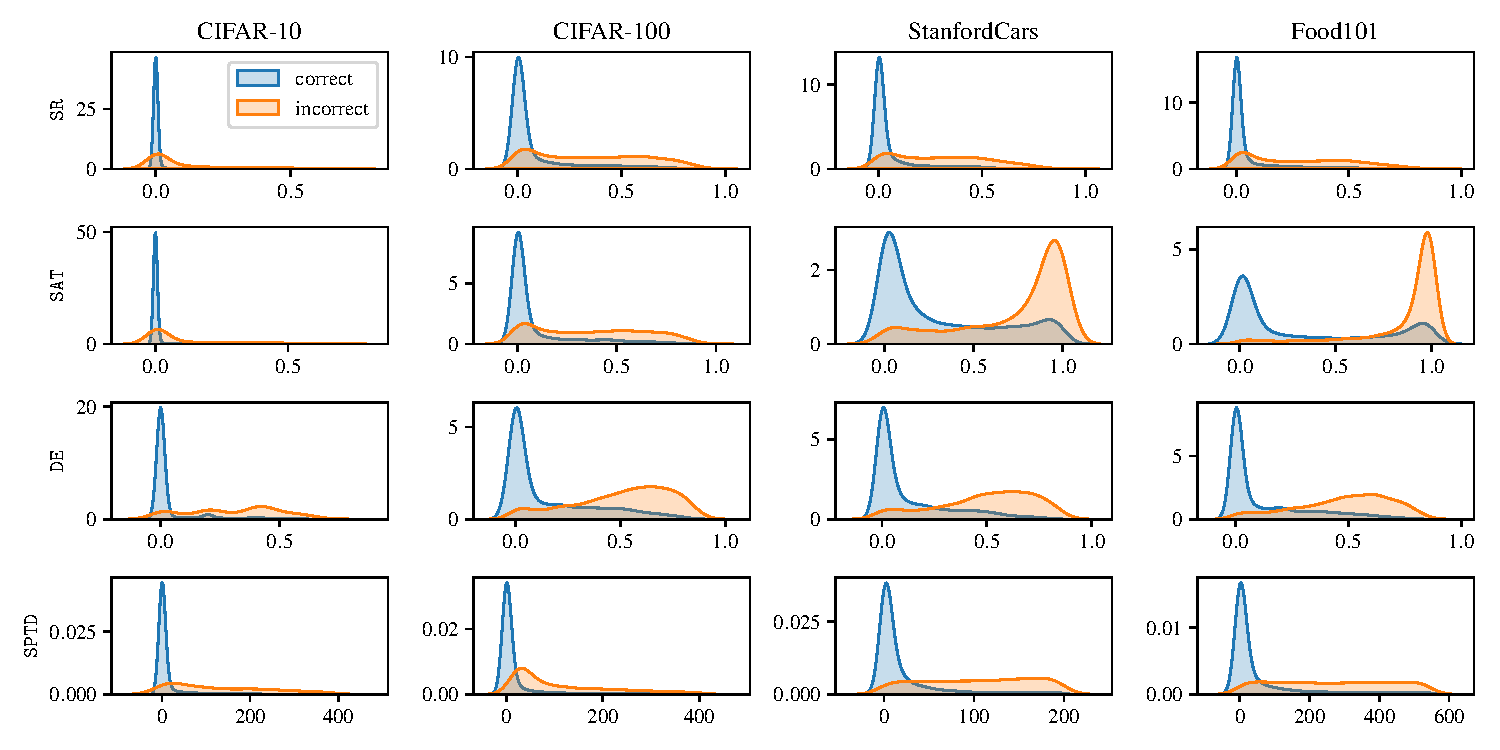
\includegraphics[width=\linewidth]{figs/sptd/g_dists.pdf}
% \caption{\newlyadded{\textbf{Extended scores for correct and incorrect data points.}  Since all methods are designed to address the selective prediction problem, they all manage to separate correct from incorrect points (albeit at varying success rates). We see that \sptd spreads the scores for incorrect points over a wide range with little overlap. We observe that for \sr, incorrect and correct points both have their mode at approximately the same location which hinders performative selective classification. Although \sat and \de show larger bumps at larger score ranges, the separation with correct points is weaker as correct points also result in higher scores more often than for \sptd. }}
% \label{fig:scores_ext}
% \end{figure*}

% }
\subsubsection{CIFAR-100 Results With ResNet-50}

We further provide a full set of results using the larger ResNet-50 architecture on CIFAR-100 in Figure~\ref{tab:cifar100_res50}.

\begin{table*}[t]
    \centering {
            \caption[Selective accuracy achieved across coverage levels for CIFAR-100 with ResNet-50.]{\textbf{Selective accuracy achieved across coverage levels for CIFAR-100 with ResNet-50}.}
    \vspace{5pt}
    \label{tab:cifar100_res50}

    \begin{tabular}{cccccc}
\toprule
Cov. &       \sr &       \satersr &      \de &      \sptd &        \sptdde \\
\midrule
  100 &  \underline{\bfseries 77.0 (±0.0)} &  \underline{\bfseries 77.0 (±0.0)} &  \bfseries 77.0 (±0.0) &  \underline{\bfseries 77.0 (±0.0)} &  \bfseries 77.0 (±0.0) \\
90 & 79.2 (± 0.1) & 79.9 (± 0.1) & 81.2 (± 0.0) & \underline{81.4 (± 0.1)} & \bfseries 82.1 (± 0.1) \\
80 & 83.1 (± 0.0) & 83.9 (± 0.0) & 85.7 (± 0.1) & \underline{85.6 (± 0.1)} & \bfseries 86.0 (± 0.2) \\
70 & 87.4 (± 0.1) & 88.2 (± 0.1) & 89.6 (± 0.1) & \underline{\textbf{89.7 (± 0.0)}} & \bfseries 89.8 (± 0.1) \\
60 & 90.5 (± 0.0) & 90.8 (± 0.2) & \bfseries{90.7 (± 0.2)} & \underline{90.6 (± 0.0)} & \bfseries 90.9 (± 0.1) \\
50 & 93.4 (± 0.1) & 93.8 (± 0.0) & 95.3 (± 0.0) & \underline{95.1 (± 0.0)} & \bfseries 95.4 (± 0.0) \\
40 & 95.4 (± 0.0) & 95.5 (± 0.1) & \textbf{97.1 (± 0.1)} & \underline{\textbf{97.2 (± 0.1)}} & \bfseries 97.2 (± 0.0) \\
30 & 97.4 (± 0.2) & 97.7 (± 0.0) & \textbf{98.6 (± 0.1)} & \underline{\textbf{98.6 (± 0.1)}} & \bfseries 98.7 (± 0.0) \\
20 & 97.9 (± 0.1) & 98.4 (± 0.1) & 99.0 (± 0.0) & \underline{99.2 (± 0.1)} & \bfseries 99.2 (± 0.1) \\
10 & 98.1 (± 0.0) & 98.8 (± 0.1) & 99.2 (± 0.1) & \underline{\textbf{99.4 (± 0.1)}} & \bfseries 99.6 (± 0.1) \\
\bottomrule
\end{tabular}
}
\end{table*}

\subsubsection{Applying \sptd on Top of \sat}
\label{sec:sptd_on_sat}

Our main set of results suggest that applying \sptd on top of \de further improves performance. The same effect holds when applying \sptd on top of non-ensemble-based methods such as \sat. We document this result in Figure~\ref{fig:sat_sptd}. 

\begin{figure*}[t]
  \centering
  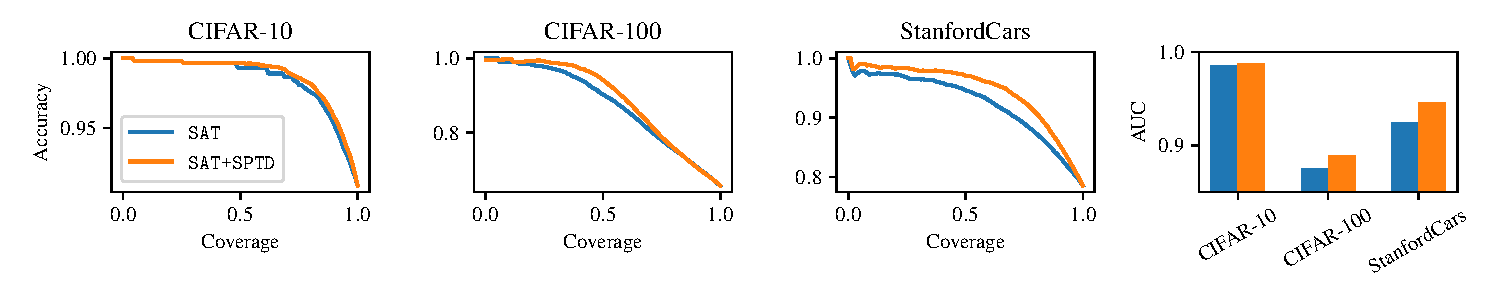
\includegraphics[width=\linewidth]{figs/sptd/sat+sptd.pdf}
\caption[Applying \sptd on top of \sat.]{\textbf{Applying \sptd on top of \sat.} Similar as with \de, we observe that the application of \sptd improves performance.}
\label{fig:sat_sptd}
\end{figure*}


\subsubsection{Ablation on $k$}

We provide a comprehensive ablation on the weighting parameter $k$ in Figures~\ref{fig:weighting} and~\ref{fig:k_ext}.

\begin{figure*}[t]
  \centering
  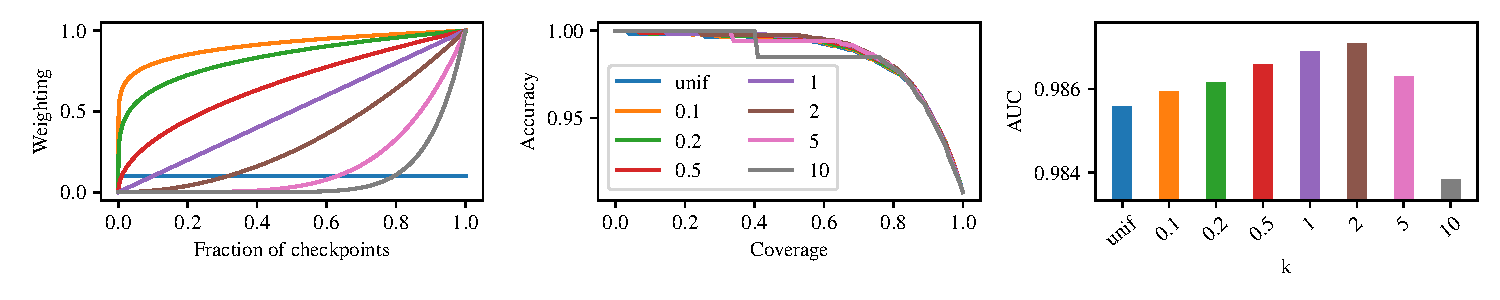
\includegraphics[width=\linewidth]{figs/sptd/k_ext.pdf}
\caption[Extended ablation results on $k$ on CIFAR-10.]{\textbf{Extended ablation results on $k$ on CIFAR-10.} We now also consider $k \in (0,1]$ as well as a uniform weighting assigning the same weight to all checkpoints. We confirm that a convex weighting yields best performance.}
\label{fig:k_ext}
\end{figure*}

\subsubsection{Comparison With Logit-Variance Approaches}


We showcase the effectiveness of \sptd against \logitvar~\citep{swayamdipta2020dataset}, an approach that also computes predictions of intermediate models but instead computes the variance of the correct prediction. We adapt this method to our selective prediction approach (for which true labels are not available) by computing the variance over the maximum predicted logit instead of the true logit. In Figure~\ref{fig:logitvar}, we see that the weighting of intermediate checkpoints introduced by \sptd leads to stronger performance over the \logitvar baseline approach. 

\begin{figure*}[t]
  \centering
  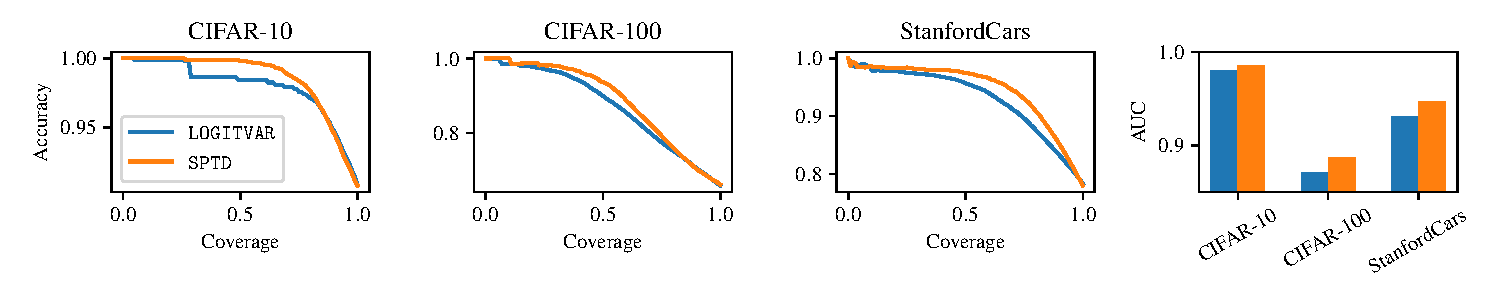
\includegraphics[width=\linewidth]{figs/sptd/logitvariance.pdf}
\caption[Comparison of \logitvar vs \sptd.]{\textbf{Comparison of \logitvar vs \sptd.} We observe that \sptd, which incorporates weighting of intermediate checkpoints using $v_t$, outperforms \logitvar.
}
\label{fig:logitvar}
\end{figure*}

\subsubsection{Estimating $\tau$ on Validation VS Test Data}

Consistent with prior works \citep{geifman2017selective, liu2019deep, huang2020self, feng2023towards}, we estimate $\tau$ directly on the test set. However, a realistically deployable approach has to compute thresholds based on a validation set for which labels are available. In the case of selective classification, the training, validation, and test sets follow the i.i.d. assumption, which means that an approach that sets the threshold based on a validation set should work performantly on a test set, too. Under consistent distributional assumptions, estimating thresholds on a validation set functions as an unbiased estimator of accuracy/coverage tradeoffs on the test set. By the same virtue, setting thresholds directly on the test set and observing the SC performance on that test set should be indicative for additional test samples beyond the actual provided test set. It is important to remark that the validation set should only be used for setting the thresholds and not for model selection / early stopping which would indeed cause a potential divergence between SC performance on the validation and test sets. Further note that violations of the i.i.d assumption can lead to degraded performance due to mismatches in attainable coverage as explored in~\cite{bar2023window}.

To confirm this intuition, we present an experiment in Figure~\ref{fig:train_test} and Figure~\ref{fig:train_test_sat} where we select 50\% of the samples from the test set as our validation set (and maintain the other 50\% of samples as our new test set). We first generate 5 distinct such validation-test splits, set the thresholds for $\tau$ based on the validation set, and then evaluate selective classification performance on the test set by using the thresholds derived from the validation set. We compare these results with our main approach which sets the thresholds based on the test set directly (ignoring the validation set). We provide an additional experiment where we partition the validation set from the training set in Figure~\ref{fig:train_test_nntd_train}. We see that the results are statistically indistinguishable from each other, confirming that this evaluation practice is valid for the selective classification setup we consider. 

\begin{figure*}[t]
  \centering
  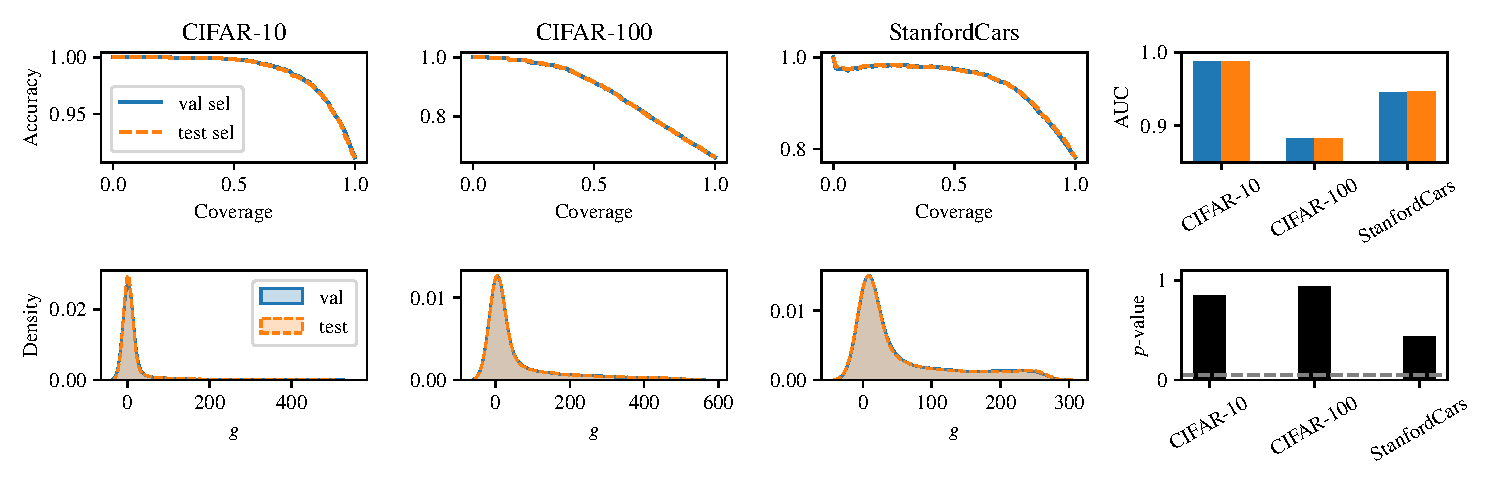
\includegraphics[width=\linewidth]{figs/sptd/train_test_nntd.pdf}
\caption[\sptd accuracy/coverage trade-offs and score distributions on test data obtained by computing $\tau$ on a validation set or directly on the test set.]{\textbf{\sptd accuracy/coverage trade-offs and score distributions on test data obtained by computing $\tau$ on a validation set or directly on the test set.} The first row shows the obtained accuracy/coverage trade-offs with the respective AUC scores. In the second row, we show the score distribution for both the picked validation and test sets, along with $p$-values from a KS-test to determine the statistical closeness of the distributions. Overall, we observe that both methods are statistically indistinguishable from each other. 
}
\label{fig:train_test}
\end{figure*}

\begin{figure*}[t]
  \centering
  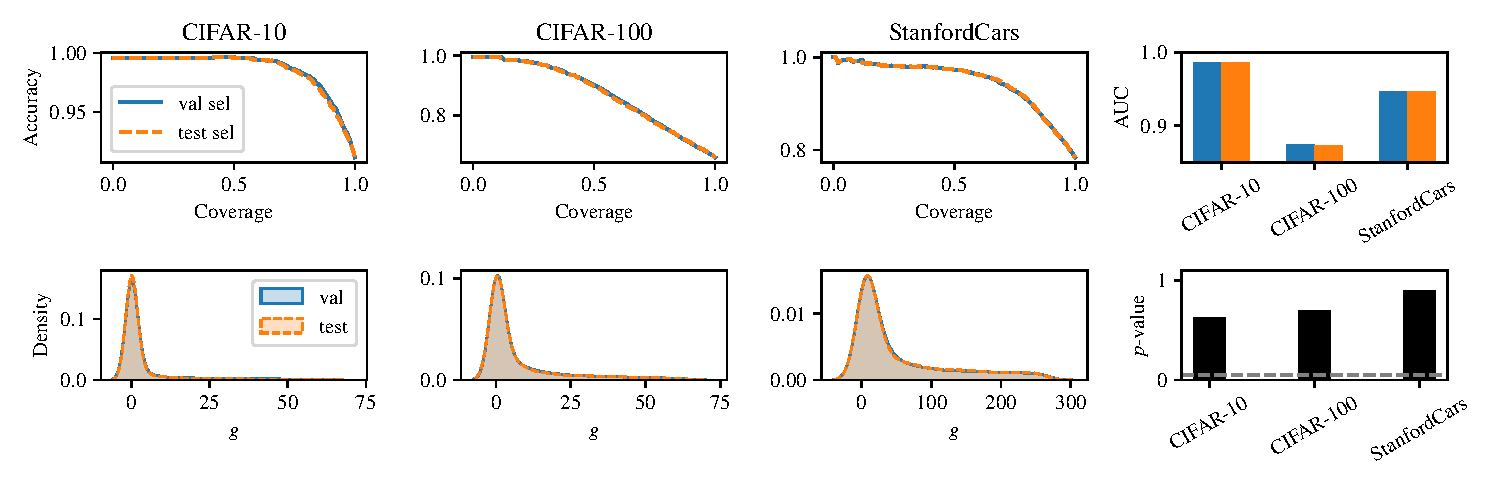
\includegraphics[width=\linewidth]{figs/sptd/train_test_sat.pdf}
\caption[\sat accuracy/coverage trade-offs and score distributions on test data obtained by computing $\tau$ on a validation set or directly on the test set.]{\textbf{\sat accuracy/coverage trade-offs and score distributions on test data obtained by computing $\tau$ on a validation set or directly on the test set.} Same as Figure~\ref{fig:train_test} but with \sat.
}
\label{fig:train_test_sat}
\end{figure*}

\begin{figure*}[t]
  \centering
  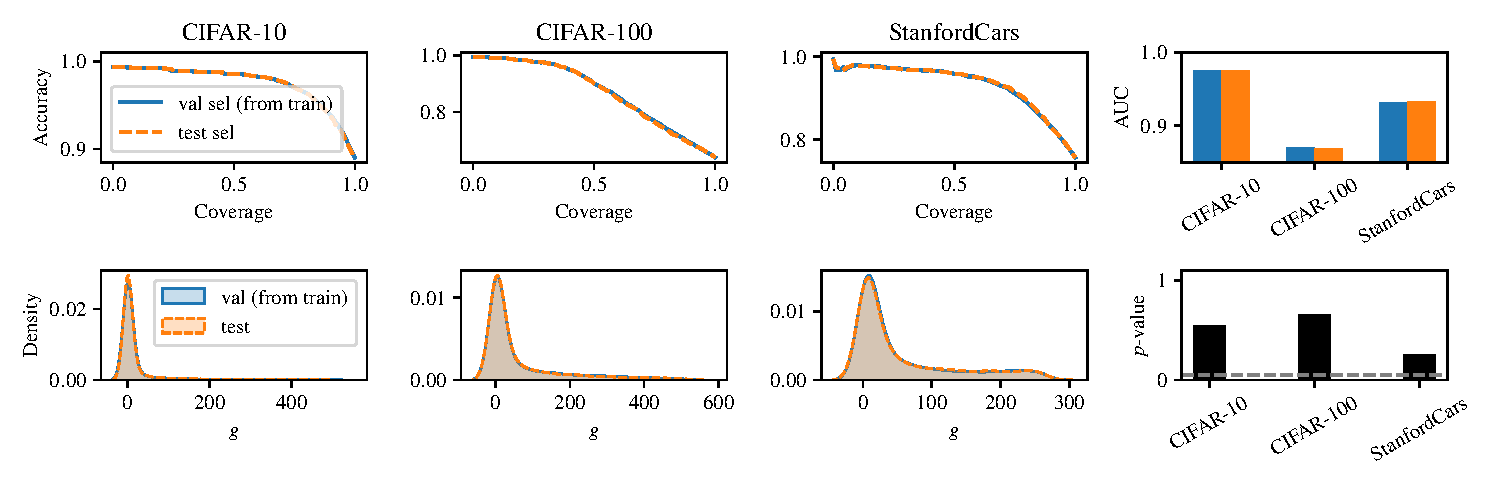
\includegraphics[width=\linewidth]{figs/sptd/train_test_nntd_train.pdf}
\caption[\sptd accuracy/coverage trade-offs and score distributions on test data obtained by computing $\tau$ on a validation set or directly on the test set.]{\textbf{\sptd accuracy/coverage trade-offs and score distributions on test data obtained by computing $\tau$ on a validation set or directly on the test set.} Same as Figure~\ref{fig:train_test} but with the validation set is taken from the original training set.
}
\label{fig:train_test_nntd_train}
\end{figure*}

\begin{figure*}[t]
\centering
  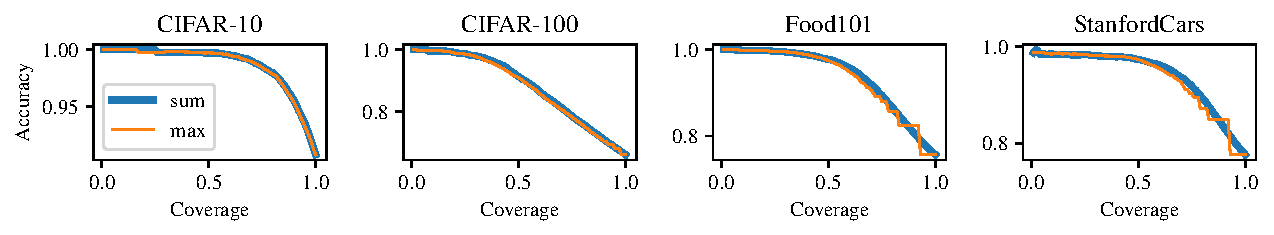
\includegraphics[width=\linewidth]{figs/sptd/max_sum.pdf}
\caption[\textbf{Comparing \smax and \ssum performance}. It is clear that \ssum effectively denoises \smax.]{\textbf{Comparing \smax and \ssum performance}. It is clear that \ssum effectively denoises \smax.}
\label{fig:sum_v_max}
\end{figure*}

\subsubsection{Comparing \smax and \ssum}
\label{sec:max_v_sum}

As per our theoretical framework and intuition provided in Section~\ref{sec:method}, the sum score~\ssum should offer the most competitive selective classification performance. We confirm this finding in Figure~\ref{fig:sum_v_max} where we plot the accuracy/coverage curves across all datasets for both \smax and \ssum. Overall, we find that the sum score~\ssum consistently outperforms the more noisy maximum score~\smax.

\begin{figure}[t]
\vspace{-5pt}
\centering

\begin{subfigure}[b]{0.23\linewidth}
  \centering
  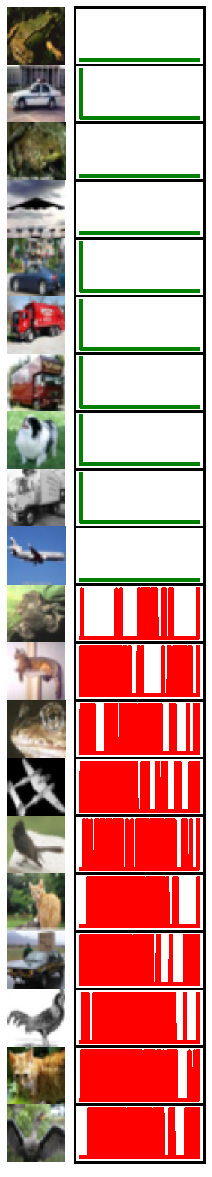
\includegraphics[width=\linewidth]{figs/sptd/cifar10_points_ext.pdf}
  % \caption{CIFAR-10}
\end{subfigure}
\hfill
\begin{subfigure}[b]{0.23\linewidth}
  \centering
  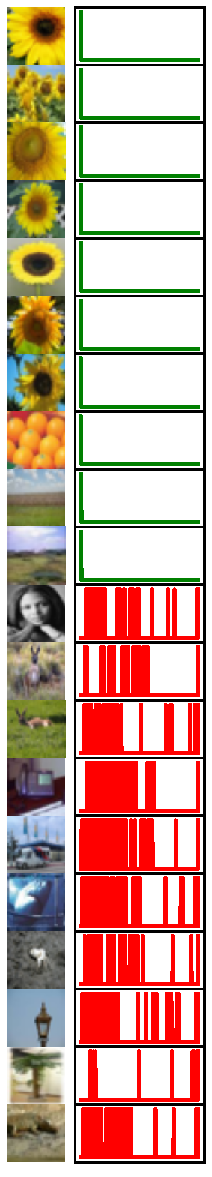
\includegraphics[width=\linewidth]{figs/sptd/cifar100_points_ext.pdf}
  % \caption{CIFAR-100}
\end{subfigure}
\hfill
\begin{subfigure}[b]{0.23\linewidth}
  \centering
  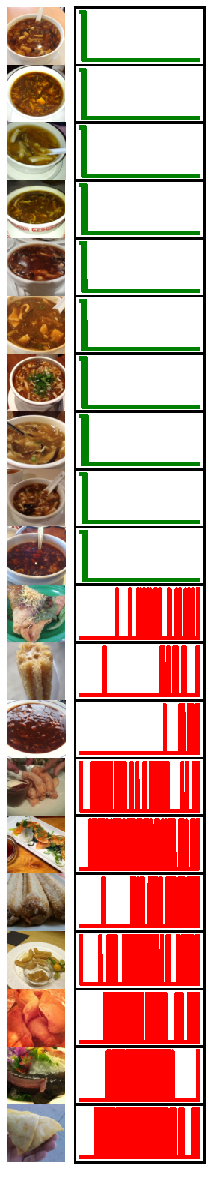
\includegraphics[width=\linewidth]{figs/sptd/food_points_ext.pdf}
  % \caption{Food101}
\end{subfigure}
\hfill
\begin{subfigure}[b]{0.23\linewidth}
  \centering
  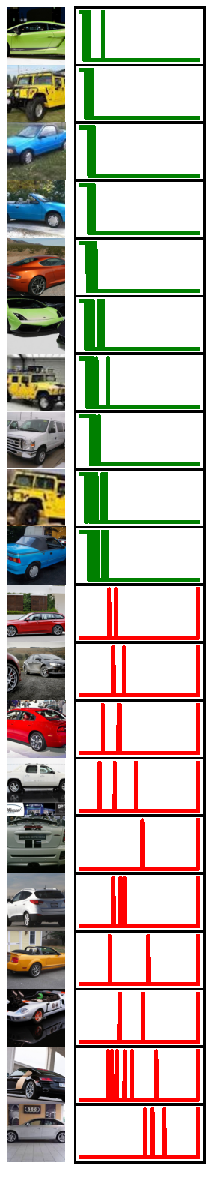
\includegraphics[width=\linewidth]{figs/sptd/cars_points_ext.pdf}
  % \caption{Stanford Cars}
\end{subfigure}

\caption[\textbf{Additional individual examples across datasets.}]{\textbf{Additional individual examples across datasets.}}
\label{fig:indiv_ex_ext}
\end{figure}


\subsection{The Importance of Accuracy Alignment}

Our results in Table~\ref{tab:target_cov} rely on accuracy alignment: We explicitly make sure to compare all methods on an equal footing by disentangling selective prediction performance from gains in overall utility. This is done by early stopping model training when the accuracy of the worst performing model is reached.

We expand on the important point that many previous approaches conflate both (i) generalization performance and (ii) selective prediction performance into a single score: the area under the accuracy/coverage curve. This metric can be maximized either by improving generalization performance (choosing different architectures or model classes) or by actually improving the ranking of points for selective prediction (accepting correct points first and incorrect ones last). As raised by a variety of recent works \cite{geifman2018bias, rabanser2023training, cattelan2023improving}, it is impossible and problematic to truly assess whether a method performs better at selective prediction (i.e., determining the correct acceptance ordering) without normalizing for this inherent difference yielded as a side effect by various SC methods. In other words, an SC method with lower base accuracy (smaller correct set) can still outperform another SC method with higher accuracy (larger correct set) in terms of the selective acceptance ordering (an example of which is given in Table 3 of \cite{liu2019deep}). Accuracy normalization allows us to eliminate these confounding effects between full-coverage utility and selective prediction performance by identifying which models are better at ranking correct points first and incorrect ones last. This is of particular importance when comparing selective prediction methods which change the training pipeline in different ways, as is done in the methods presented in Table~\ref{tab:target_cov}.

However, when just comparing \sptd to one other method, we do not need to worry about accuracy normalization. Showcasing this, we run \sptd on top of an unnormalized \satersr run and provide these experiments in Figure~\ref{fig:sat_sptd}. We see that the application of \sptd on top of \satersr allows us to further boost performance (similar to the results where we apply \sptd on top of \de in Table~\ref{tab:target_cov}). So to conclude, experimentally, when using the best model, we see that \sptd still performs better at selective prediction than the relevant baseline for that training pipeline. We wish to reiterate that this issue of accuracy normalization highlights another merit of \sptd, which is that it can easily be applied on top of any training pipeline (including those that lead to the best model) and allows easy comparison to the selective classification method that training pipeline was intended to be deployed with.

\subsection{Evaluation using other performance metrics}

We further provide results of summary performance metrics across datasets in Table~\ref{tab:sc_evals}:

\begin{itemize}
    \item The area under the accuracy-coverage curve (\texttt{AUACC}) as discussed in \citet{geifman2018bias}.
    \item The area under the receiver operating characteristic (\texttt{AUROC}) as suggested by \citet{galil2023can}.
    \item The accuracy normalized selective classification score (\texttt{ANSC}) from~\citet{geifman2018bias} and ~\citet{rabanser2023training}.
\end{itemize}

\begin{table}[ht]
\centering
\caption{\textbf{Evaluation of SC approaches using various evaluation metrics}. }
\label{tab:sc_evals}
\begin{tabular}{ccccc}
\toprule
Dataset & Method & $1-\texttt{AUACC}$ & \texttt{ANSC} & \texttt{AUROC} \\
\midrule
\multirow{5}{*}{CIFAR10} & \texttt{SR} & 0.053 $\pm$ 0.002 & 0.007 $\pm$ 0.000 & 0.918 $\pm$ 0.002 \\
& \texttt{SPTD} & 0.048 $\pm$ 0.001 & 0.004 $\pm$ 0.000 & 0.938 $\pm$ 0.002 \\
& \texttt{DE} & 0.046 $\pm$ 0.002 & 0.004 $\pm$ 0.000 & 0.939 $\pm$ 0.003 \\
& \texttt{SAT} & 0.054 $\pm$ 0.002 & 0.006 $\pm$ 0.000 & 0.924 $\pm$ 0.005 \\
& \texttt{DG} & 0.054 $\pm$ 0.001 & 0.006 $\pm$ 0.000 & 0.922 $\pm$ 0.005 \\
\midrule
\multirow{5}{*}{CIFAR100} & \texttt{SR} & 0.181 $\pm$ 0.001 & 0.041 $\pm$ 0.001 & 0.865 $\pm$ 0.003 \\
& \texttt{SPTD} & 0.174 $\pm$ 0.002 & 0.037 $\pm$ 0.000 & 0.872 $\pm$ 0.002 \\
& \texttt{DE} & 0.159 $\pm$ 0.001 & 0.030 $\pm$ 0.001 & 0.880 $\pm$ 0.003 \\
& \texttt{SAT} & 0.180 $\pm$ 0.001 & 0.041 $\pm$ 0.001 & 0.866 $\pm$ 0.003 \\
& \texttt{DG} & 0.182 $\pm$ 0.001 & 0.041 $\pm$ 0.001 & 0.867 $\pm$ 0.002 \\
\midrule
\multirow{5}{*}{GTSRB} & \texttt{SR} & 0.020 $\pm$ 0.002 & 0.001 $\pm$ 0.000 & 0.986 $\pm$ 0.003 \\
& \texttt{SPTD} & 0.019 $\pm$ 0.002 & 0.001 $\pm$ 0.000 & 0.986 $\pm$ 0.005 \\
& \texttt{DE} & 0.015 $\pm$ 0.001 & 0.001 $\pm$ 0.000 & 0.986 $\pm$ 0.002 \\
& \texttt{SAT} & 0.027 $\pm$ 0.001 & 0.001 $\pm$ 0.000 & 0.984 $\pm$ 0.002 \\
& \texttt{DG} & 0.019 $\pm$ 0.003 & 0.001 $\pm$ 0.000 & 0.986 $\pm$ 0.002 \\
\midrule
\multirow{5}{*}{SVHN} & \texttt{SR} & 0.027 $\pm$ 0.000 & 0.006 $\pm$ 0.001 & 0.895 $\pm$ 0.004 \\
& \texttt{SPTD} & 0.025 $\pm$ 0.003 & 0.003 $\pm$ 0.001 & 0.932 $\pm$ 0.005 \\
& \texttt{DE} & 0.021 $\pm$ 0.001 & 0.005 $\pm$ 0.000 & 0.912 $\pm$ 0.003 \\
& \texttt{SAT} & 0.028 $\pm$ 0.001 & 0.006 $\pm$ 0.000 & 0.895 $\pm$ 0.002 \\
& \texttt{DG} & 0.026 $\pm$ 0.001 & 0.007 $\pm$ 0.000 & 0.896 $\pm$ 0.006 \\
\bottomrule
\end{tabular}
\end{table}

\newlyadded{

\subsection{Evaluation of more competing approaches}

We further compare our method with two more contemporary selective prediction approaches:
\begin{itemize}
    \item \aucoc \citep{sangalli2024expert}: This work uses a custom cost function for multi-class classification that accounts for the trade-off between a neural network’s accuracy and the amount of data that requires manual inspection from a domain expert.
    \item \cclsc \citep{wu2024confidence}: This work proposes optimizing feature layers to reduce intra-class variance via contrastive learning.
\end{itemize}
Across both methods, we find that they do not outperform ensemble-based methods like \de and hence also do not outperform \sptd. See Table~\ref{tab:target_cov_ext} for detailed results.
}

\begin{table}[h!]
\centering
\caption[Selective accuracy achieved across coverage levels for \aucoc and \cclsc]{\textbf{Selective accuracy achieved across coverage levels for \aucoc and \cclsc}. Similar as Table~\ref{tab:target_cov}. Neither \aucoc nor \cclsc is able to outperform \de or \sptd. \textbf{Bold} numbers are best results at a given coverage level across all methods and \underline{underlined} numbers are best results for methods relying on a single training run only.}
\label{tab:target_cov_ext}
\newlyadded{
\begin{tabular}{cccccc}
\toprule
& \textbf{Coverage} & \textbf{AUCOC} & \textbf{CCL-SC} & \textbf{SPTD} & \textbf{DE} \\
\midrule
\multirow{10}{*}{\rotatebox[origin=c]{90}{\textit{CIFAR-10}}} & 
100 & \underline{\textbf{92.9}} ($\pm$0.0) & \underline{\textbf{92.9}} ($\pm$0.0) & \underline{\textbf{92.9}} ($\pm$0.0) & \textbf{92.9} ($\pm$0.0) \\
& 90  & 96.0 ($\pm$0.1) & 95.9 ($\pm$0.2) & \underline{96.5} ($\pm$0.0) & \textbf{96.8} ($\pm$0.1) \\
& 80  & 98.1 ($\pm$0.2) & 98.0 ($\pm$0.3) & \underline{98.4} ($\pm$0.1) & \textbf{98.7} ($\pm$0.0) \\
& 70  & 99.0 ($\pm$0.3) & 98.5 ($\pm$0.2) & \underline{99.2} ($\pm$0.1) & \textbf{99.4} ($\pm$0.1) \\
& 60  & 99.3 ($\pm$0.1) & 99.1 ($\pm$0.2) & \underline{\textbf{99.6}} ($\pm$0.2) & \textbf{99.6} ($\pm$0.1) \\
& 50  & 99.4 ($\pm$0.2) & 99.0 ($\pm$0.3) & \underline{\textbf{99.8}} ($\pm$0.0) & 99.7 ($\pm$0.0) \\
& 40  & 99.5 ($\pm$0.1) & 99.4 ($\pm$0.2) & \underline{\textbf{99.8}} ($\pm$0.1) & \textbf{99.8} ($\pm$0.0) \\
& 30  & 99.5 ($\pm$0.2) & 99.2 ($\pm$0.3) & \underline{\textbf{99.8}} ($\pm$0.1) & \textbf{99.8} ($\pm$0.0) \\
& 20  & 99.6 ($\pm$0.1) & 99.4 ($\pm$0.2) & \underline{\textbf{100.0}} ($\pm$0.0) & 99.8 ($\pm$0.0) \\
& 10  & 99.7 ($\pm$0.0) & 99.4 ($\pm$0.1) & \underline{\textbf{100.0}} ($\pm$0.0) & 99.8 ($\pm$0.0) \\
\midrule
\multirow{10}{*}{\rotatebox[origin=c]{90}{\textit{CIFAR-100}}} &
100 & \underline{\textbf{75.1}} ($\pm$0.0) & \underline{\textbf{75.1}} ($\pm$0.0) & \underline{\textbf{75.1}} ($\pm$0.0) & \underline{\textbf{75.1}} ($\pm$0.0) \\
& 90  & 78.7 ($\pm$0.2) & 76.5 ($\pm$0.3) & \underline{\textbf{80.4}} ($\pm$0.0) & 80.2 ($\pm$0.0) \\
& 80  & 83.2 ($\pm$0.1) & 82.2 ($\pm$0.2) & \underline{\textbf{84.6}} ($\pm$0.1) & \textbf{84.7} ($\pm$0.1) \\
& 70  & 87.4 ($\pm$0.1) & 86.1 ($\pm$0.2) & \underline{\textbf{88.7}} ($\pm$0.0) & 88.6 ($\pm$0.1) \\
& 60  & 89.8 ($\pm$0.2) & 88.6 ($\pm$0.3) & \underline{90.1} ($\pm$0.0) & \textbf{90.2} ($\pm$0.2) \\
& 50  & 93.3 ($\pm$0.1) & 92.1 ($\pm$0.2) & \underline{94.6} ($\pm$0.0) & \textbf{94.8} ($\pm$0.0) \\
& 40  & 95.9 ($\pm$0.2) & 95.2 ($\pm$0.3) & \underline{\textbf{96.9}} ($\pm$0.1) & 96.8 ($\pm$0.1) \\
& 30  & 98.2 ($\pm$0.1) & 96.6 ($\pm$0.2) & \underline{\textbf{98.4}} ($\pm$0.1) & 98.4 ($\pm$0.1) \\
& 20  & 98.6 ($\pm$0.2) & 98.4 ($\pm$0.3) & \underline{98.8} ($\pm$0.2) & \textbf{99.0} ($\pm$0.0) \\
& 10  & 98.8 ($\pm$0.1) & 98.7 ($\pm$0.2) & \underline{\textbf{99.4}} ($\pm$0.1) & 99.2 ($\pm$0.1) \\
\bottomrule
\end{tabular}
}
\end{table}

% \subsubsection{Incorporating Estimates of $e_t$ into \smin and \savg}
% \label{ssec:incorp_e_t}

% Our results in \S~\ref{ssec:ver_ei_vi} show that $e_t$ is only nearly $0$ almost everywhere, we investigate whether incorporating an estimate of $e_t$ into \smin and \savg leads to additional SC improvements. Recall that in Lemma~\ref{lem:prob_accept} we gave an upper-bound on the probability that the test point is correctly classified as $\frac{v_t}{|a_t - e_t|^2}$. In the case where $e_t$ is not $0$ everywhere, we can adjust
% \begin{equation}
% 	s_\text{min} = \min_{t~s.t~a_t = 1} \frac{v_t}{|a_t - e_t|^2} \qquad \text{and} \qquad s_\text{avg} = \frac{\sum \frac{v_t}{|a_t - e_t|^2} a_t}{\sum a_t}
% \end{equation}
% accordingly. In Figure~\ref{fig:et_incorp}, we experimentally test whether incorporating an empirical estimate (first row) or a smooth decay function similar to $v_i$ (second row) robustly improve over \smin and \savg with $e_t = 0$. Our results show that neither setting outperforms our default setting with $e_t = 0$.

% \subsubsection{Performance of Jump Score \sjmp and Weighted Variance \svar}

% As discussed in Appendix~\ref{app:alt_scores}, we also investigated whether the jump score \sjmp or the weighted variance of continuous metrics \svar can be used as an effective score for SC. As we show in Figure~\ref{fig:scores_alt}, none of these metrics robustly outperforms our main method \texttt{NNTD}$(s_\text{avg}, 0.05)$.

% \subsubsection{Concave Weighting for $v_t$} As we have empirically analyzed in \S~\ref{ssec:ver_ei_vi}, the variances $v_t$ follow a monotonically decreasing and convex trend. This inspires our best performing method \texttt{NNTD}$(s_\text{avg}, 0.05)$ to use $k=0.05$ for $v_i=1-i^k$. As a sanity check, we examine whether a concave weighting yielded by $v_i=1-i^k$ for $k \geq 1$. As we demonstrate in Figure~\ref{fig:conc_weighting}, the best concave weighting is given by $k=1$. Therefore, we confirm that no concave weighting outperforms the convex weightings analyzed in Figure~\ref{fig:weighting}.

% \subsubsection{Limiting \nntd to a Subset of Last Checkpoints}
% \label{sec:add_check_strat}

% In order to determine which training stages are important for selective classification, we perform an experiment on CIFAR-10 and SVHN where we limit ourselves to a subset of the last checkpoints. In particular, we examine the coverage/error trade-off for only including the last $\{10\%,  20\%, 50\%, 80\%, 90\%, 100\%\}$ of checkpoints. We report our findings in Table~\ref{tab:perc_checkp}. We see that taking into account more than $80\%$ of checkpoints does lead to diminishing returns and that only taking into account $50\%$ or less of the total numbers of checkpoints does not lead to state-of-the-art selective classification performance. 

% \subsubsection{Selective Classification on ImageNet} In addition to our main results on CIFAR-10, CIFAR-100, SVHN, Cats \& Dogs, and GTSRB, we also provide results for our \nntd approach on ImageNet. We train a ResNet-50 over 90 epochs with an initial learning rate of 0.1, a learning rate decay of 0.1 in 30 epoch increments, momentum 0.9, and weight decay $10^{-4}$. We report our obtained accuracy/coverage trade-off in Table~\ref{tab:imagenet} and find that \nntd delivers a strong coverage/error trade-off compared to the softmax response and self-adptive training baselines.

% \subsubsection{Applying OOD Scores to Selective Classification} Finally, we also compare popular out-of-distribution detection approaches to our \nntd method. In particular, we apply three state-of-the-art approaches, namely energy-based OOD detection~(\texttt{Energy}) \citep{liu2020energy}, Mahalanobis-distance-based OOD detection~(\texttt{Mahalanobis}) \citep{lee2018simple}, and ODIN~(\texttt{ODIN}) \citep{liang2017enhancing} to the CIFAR-10 and SVHN test sets and document these results in Table~\ref{tab:ood}. Overall, we find that SOTA out-of-distribution detection techniques are not well equipped to attain SOTA selective classification performance; \nntd outperforms these methods by a large margin.

% \begin{figure}[t]
% \begin{subfigure}{.24 \linewidth}
%   \centering
%   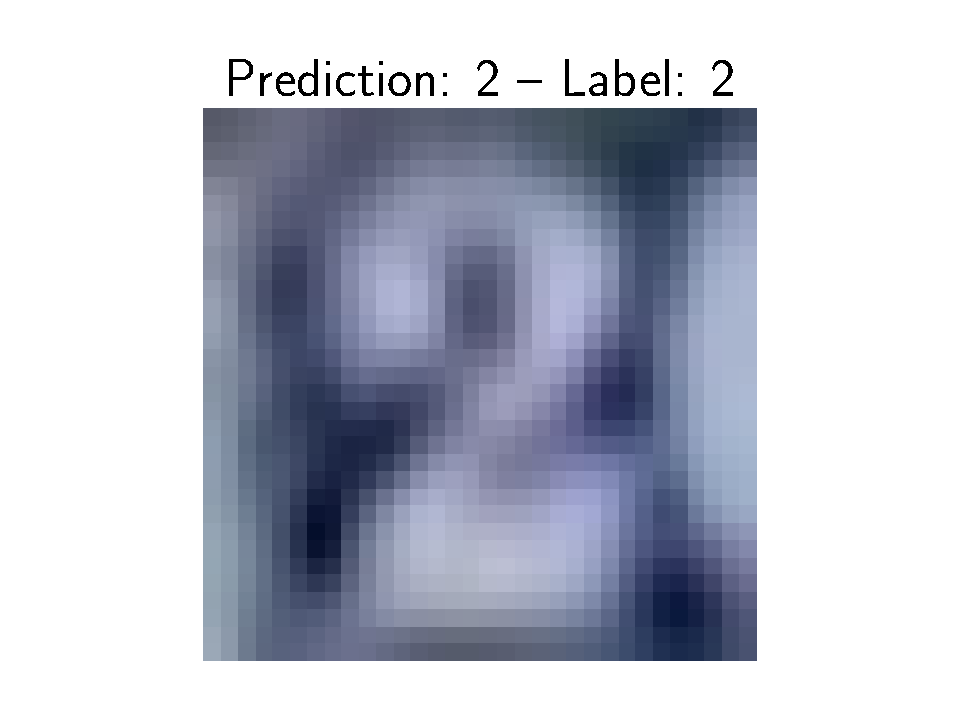
\includegraphics[width=\linewidth]{figs/sptd/svhn/data_id_20.pdf}
% \end{subfigure}
% \hfill
% \begin{subfigure}{.24 \linewidth}
%   \centering
%   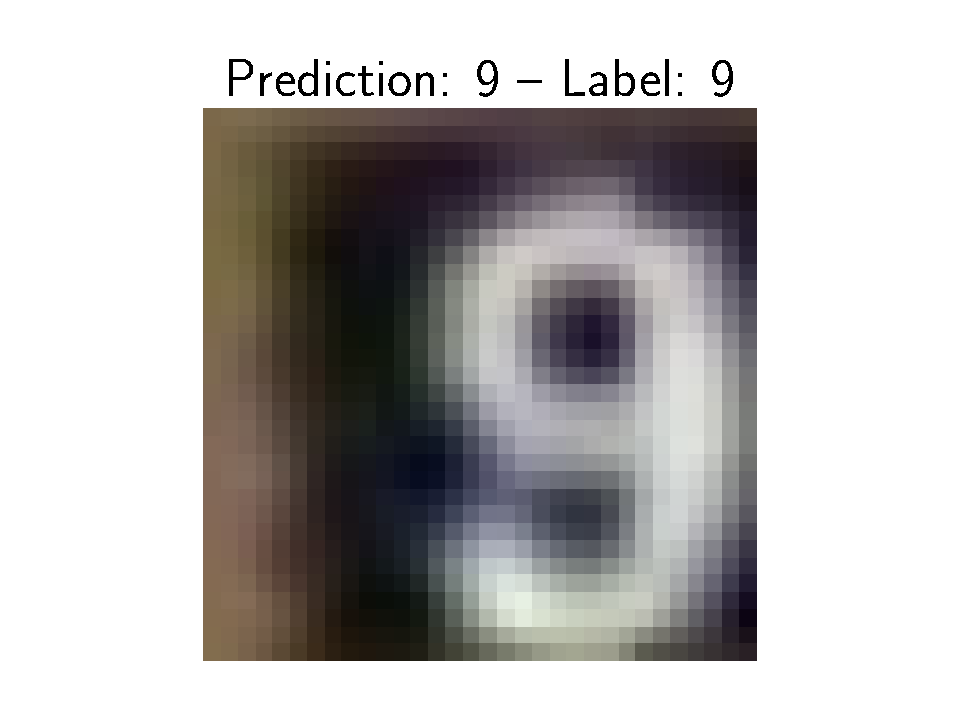
\includegraphics[width=\linewidth]{figs/sptd/svhn/data_id_43.pdf}
% \end{subfigure}
% \hfill
% \begin{subfigure}{.24 \linewidth}
%   \centering
%   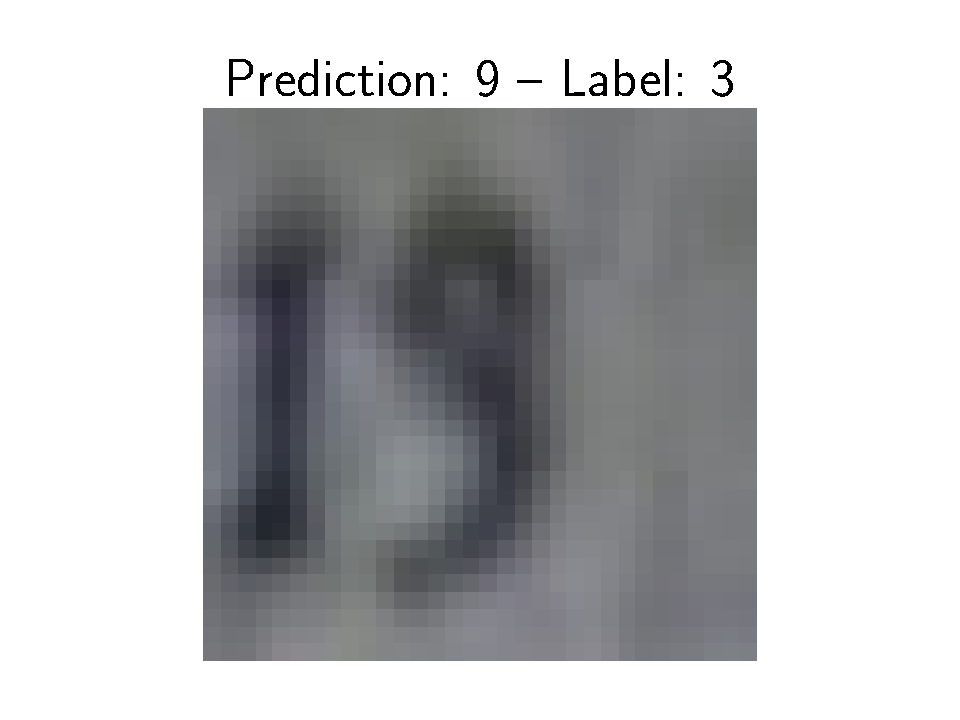
\includegraphics[width=\linewidth]{figs/sptd/svhn/data_id_23.pdf}
% \end{subfigure}
% \hfill
% \begin{subfigure}{.24 \linewidth}
%   \centering
%   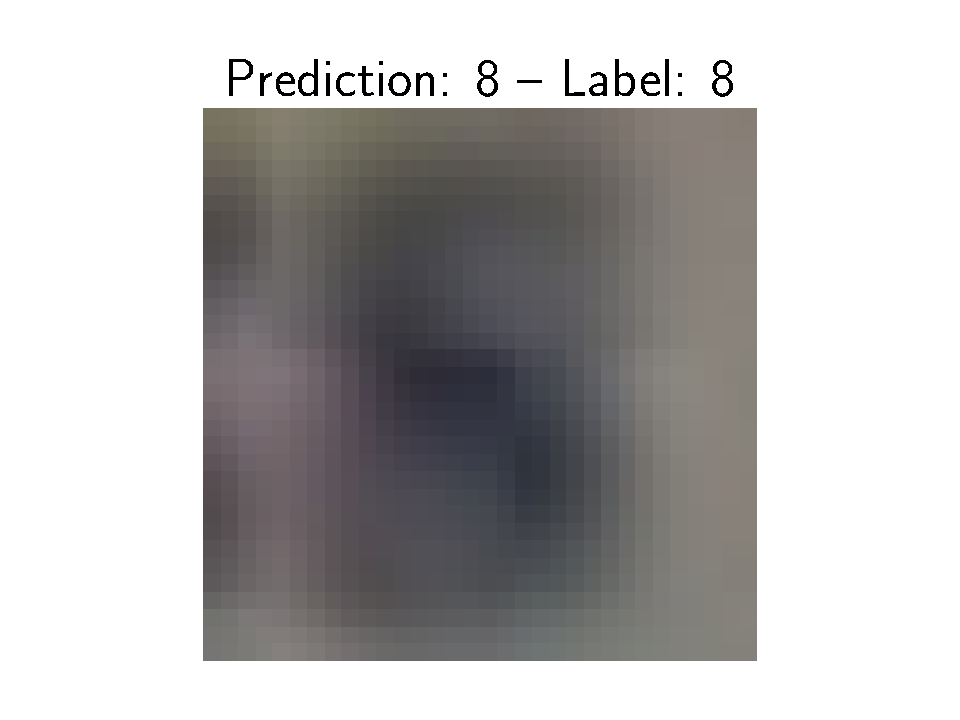
\includegraphics[width=\linewidth]{figs/sptd/svhn/data_id_32.pdf}
% \end{subfigure}

% \begin{subfigure}{.24 \linewidth}
%   \centering
%   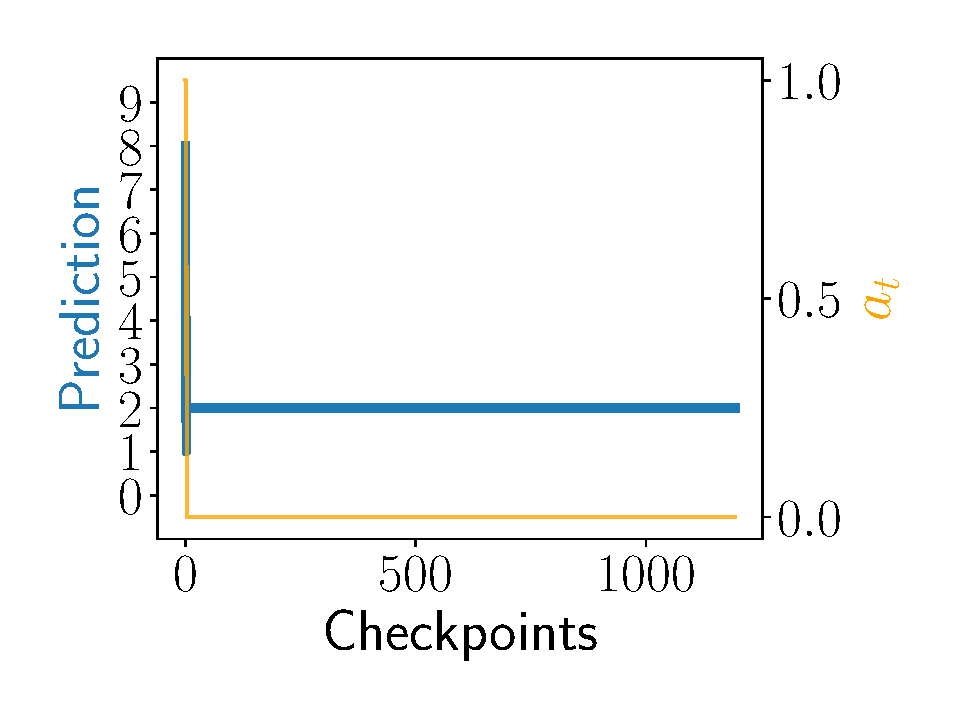
\includegraphics[width=\linewidth]{figs/sptd/svhn/metrics_id_20.pdf}
% \end{subfigure}
% \hfill
% \begin{subfigure}{.24 \linewidth}
%   \centering
%   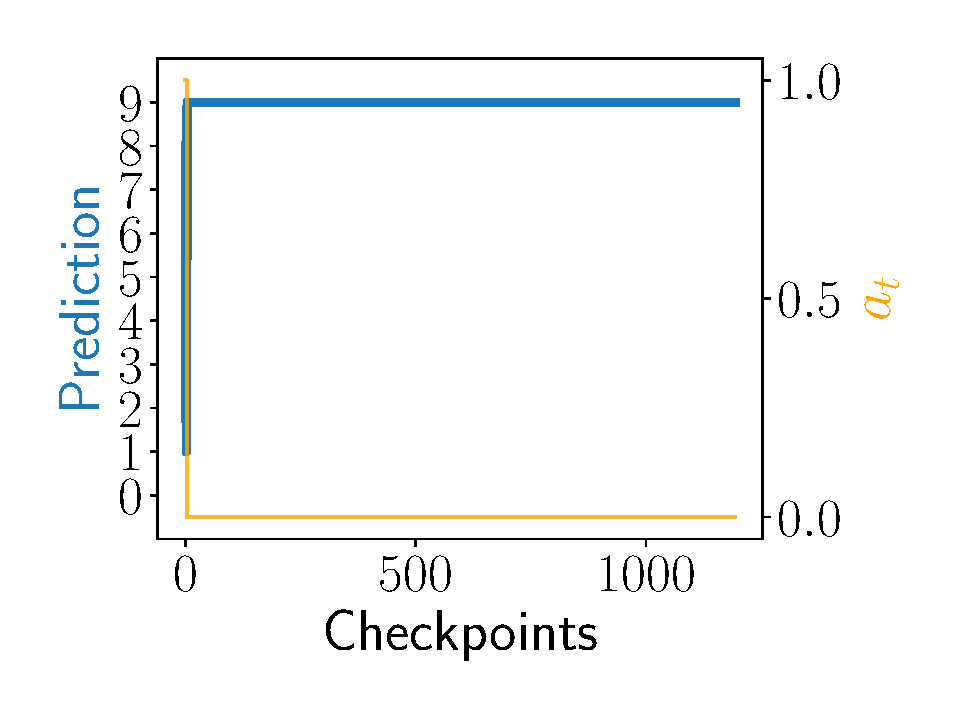
\includegraphics[width=\linewidth]{figs/sptd/svhn/metrics_id_43.pdf}
% \end{subfigure}
% \hfill
% \begin{subfigure}{.24 \linewidth}
%   \centering
%   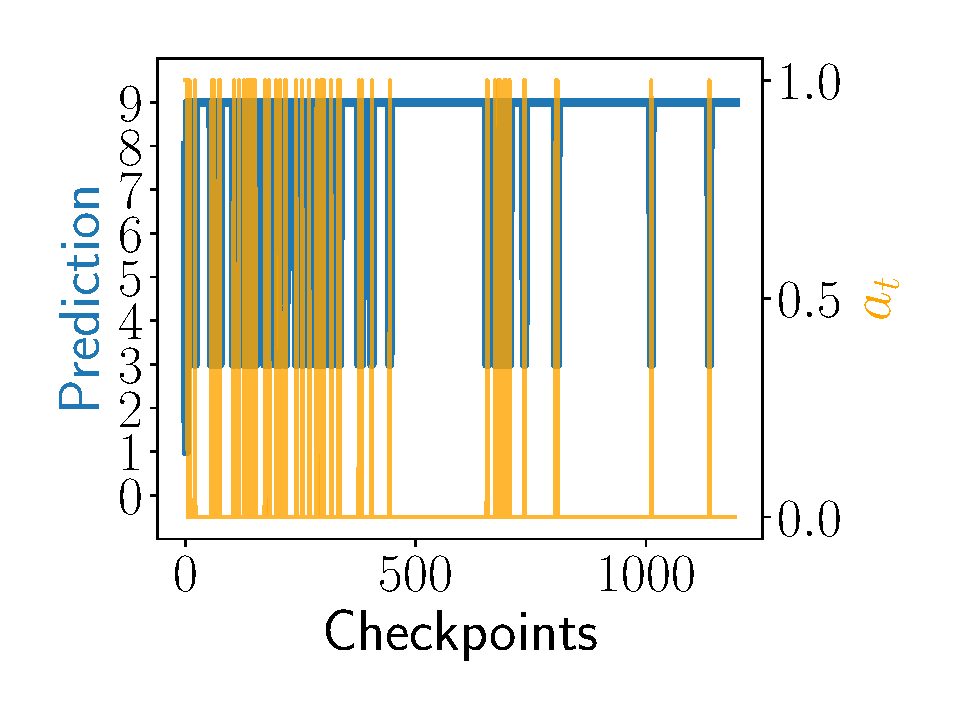
\includegraphics[width=\linewidth]{figs/sptd/svhn/metrics_id_23.pdf}
% \end{subfigure}
% \hfill
% \begin{subfigure}{.24 \linewidth}
%   \centering
%   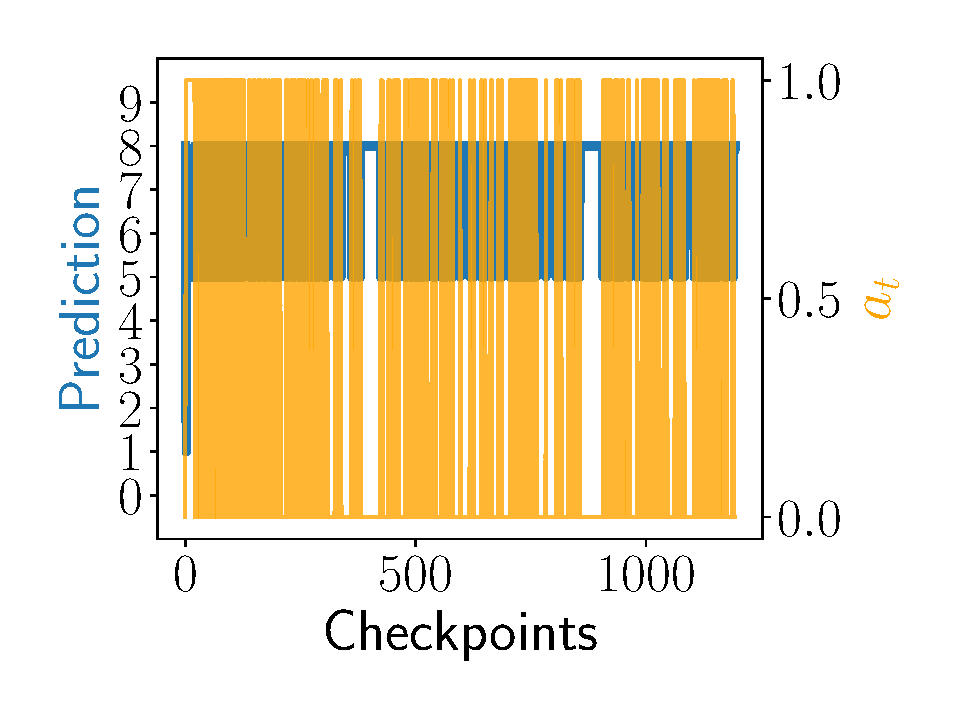
\includegraphics[width=\linewidth]{figs/sptd/svhn/metrics_id_32.pdf}
% \end{subfigure}

%  \begin{subfigure}{.24 \linewidth}
%    \centering
%    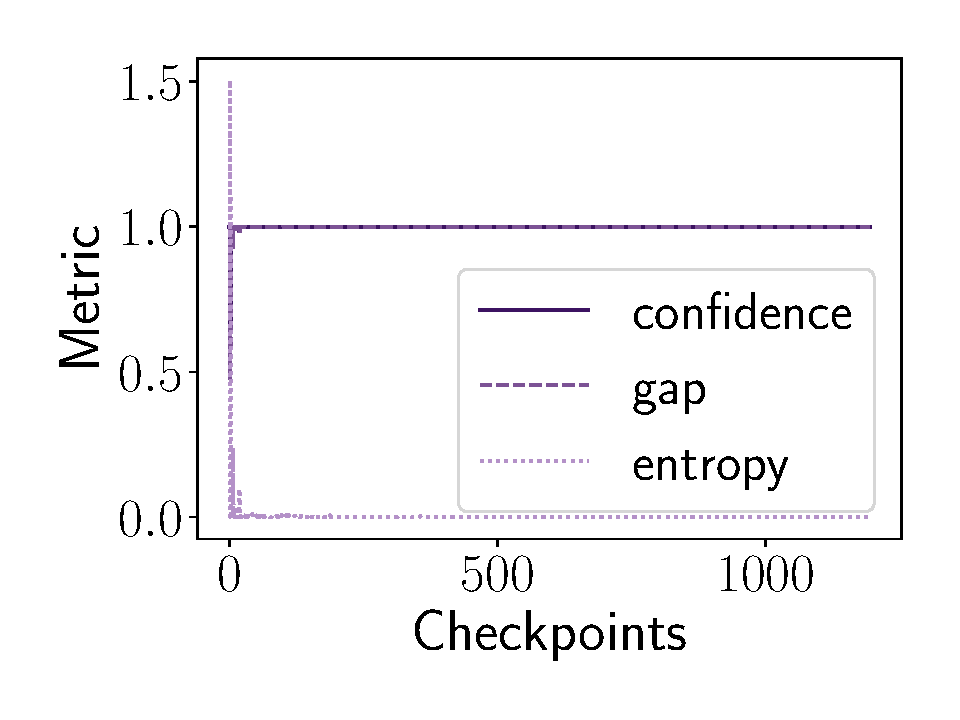
\includegraphics[width=\linewidth]{figs/sptd/svhn/metrics_alt_id_leg_20.pdf}
%  \end{subfigure}
%  \hfill
%  \begin{subfigure}{.24 \linewidth}
%    \centering
%    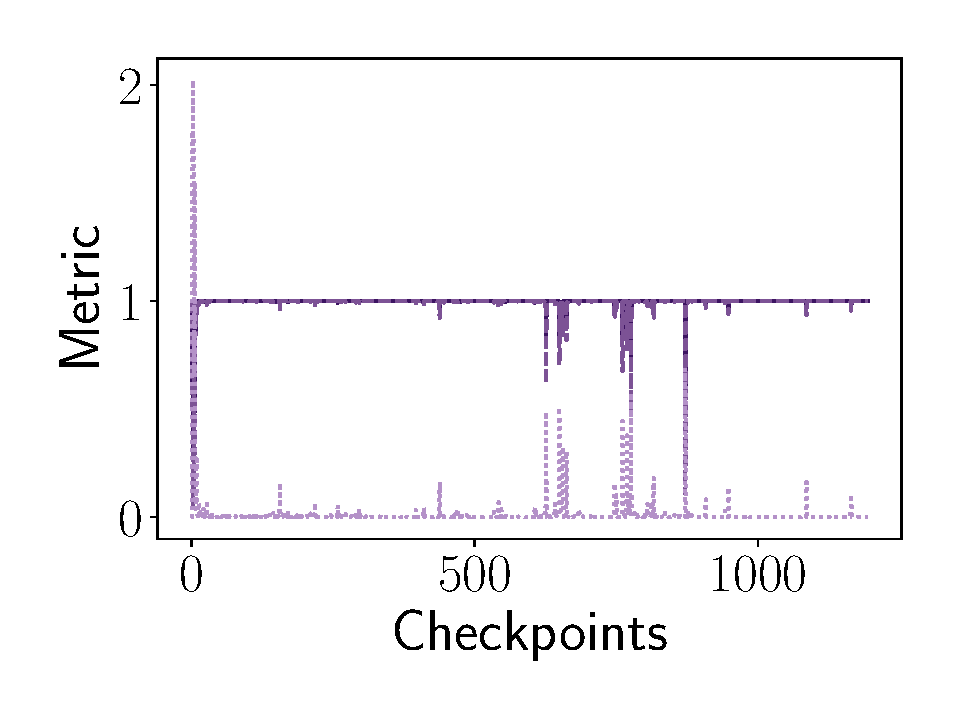
\includegraphics[width=\linewidth]{figs/sptd/svhn/metrics_alt_id_43.pdf}
%  \end{subfigure}
%  \hfill
%  \begin{subfigure}{.24 \linewidth}
%    \centering
%    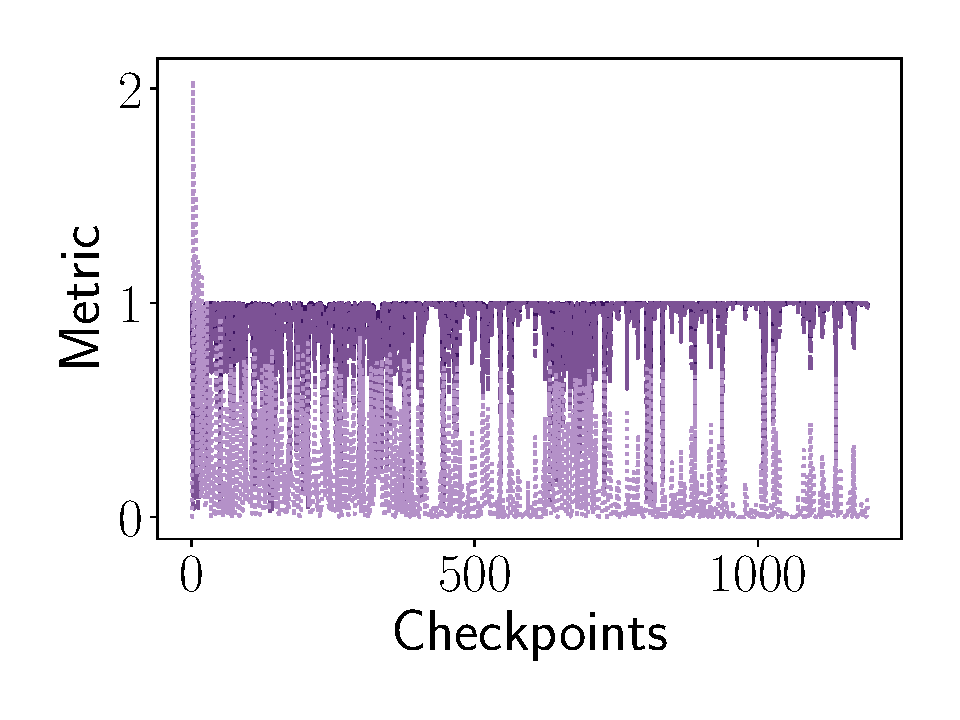
\includegraphics[width=\linewidth]{figs/sptd/svhn/metrics_alt_id_23.pdf}
%  \end{subfigure}
%  \hfill
%  \begin{subfigure}{.24 \linewidth}
%    \centering
%    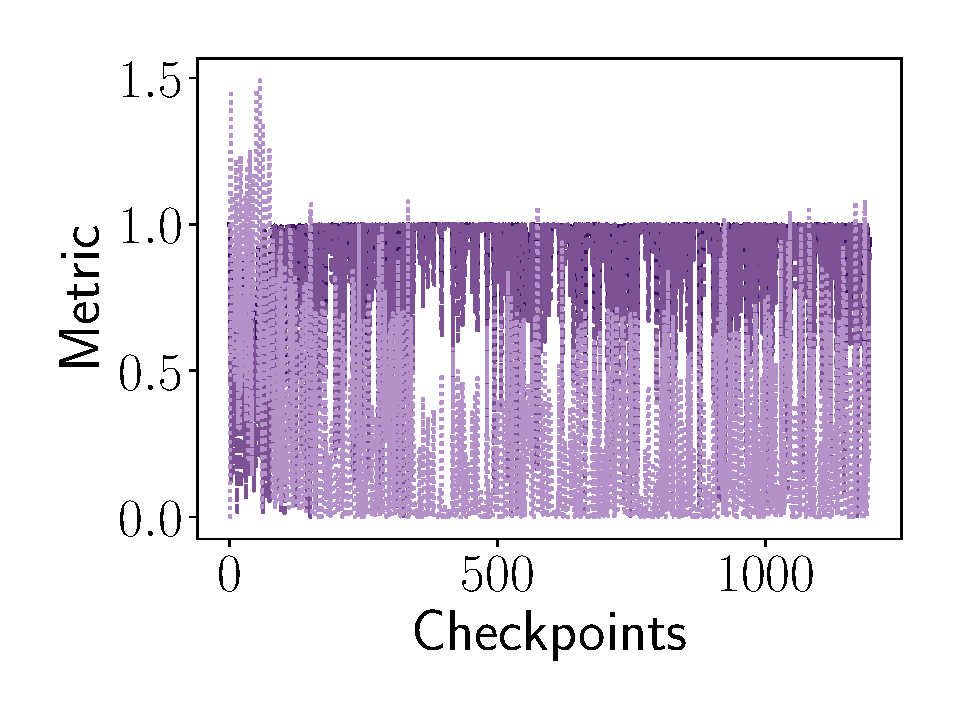
\includegraphics[width=\linewidth]{figs/sptd/svhn/metrics_alt_id_32.pdf}
%  \end{subfigure}

%  \begin{subfigure}{.24 \linewidth}
%    \centering
%    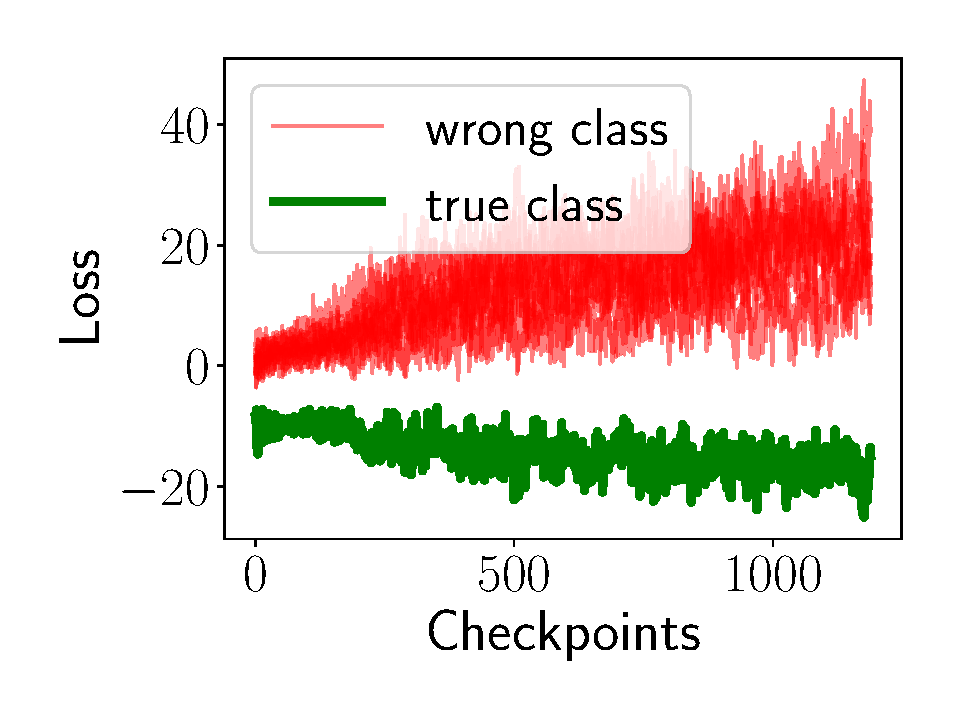
\includegraphics[width=\linewidth]{figs/sptd/svhn/losses_id_leg_20.pdf}
%  \end{subfigure}
%  \hfill
%  \begin{subfigure}{.24 \linewidth}
%    \centering
%    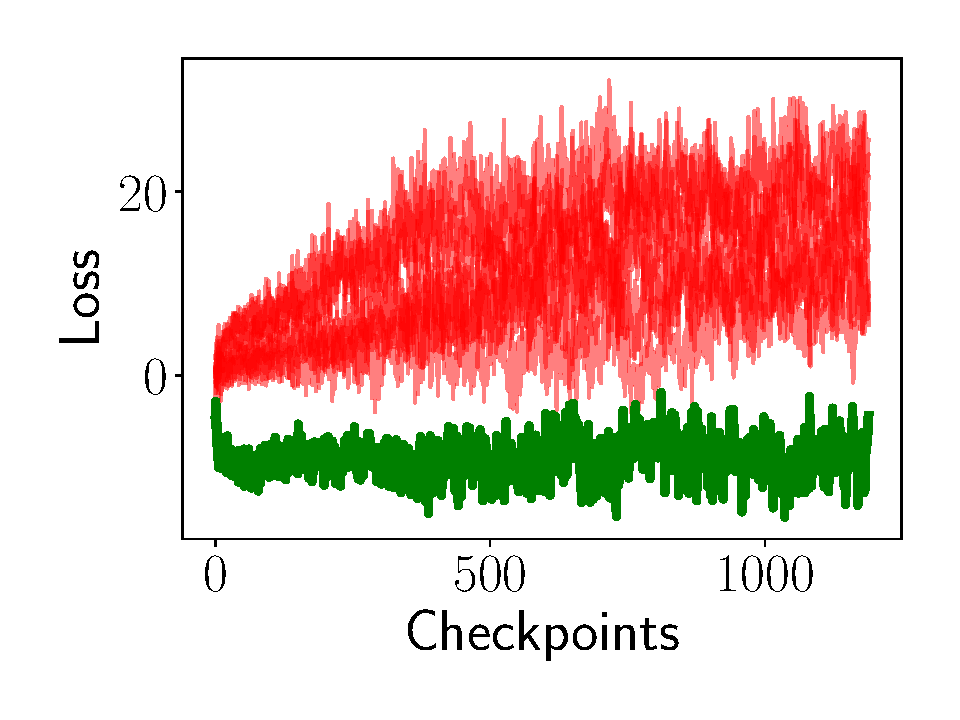
\includegraphics[width=\linewidth]{figs/sptd/svhn/losses_id_43.pdf}
%  \end{subfigure}
%  \hfill
%  \begin{subfigure}{.24 \linewidth}
%    \centering
%    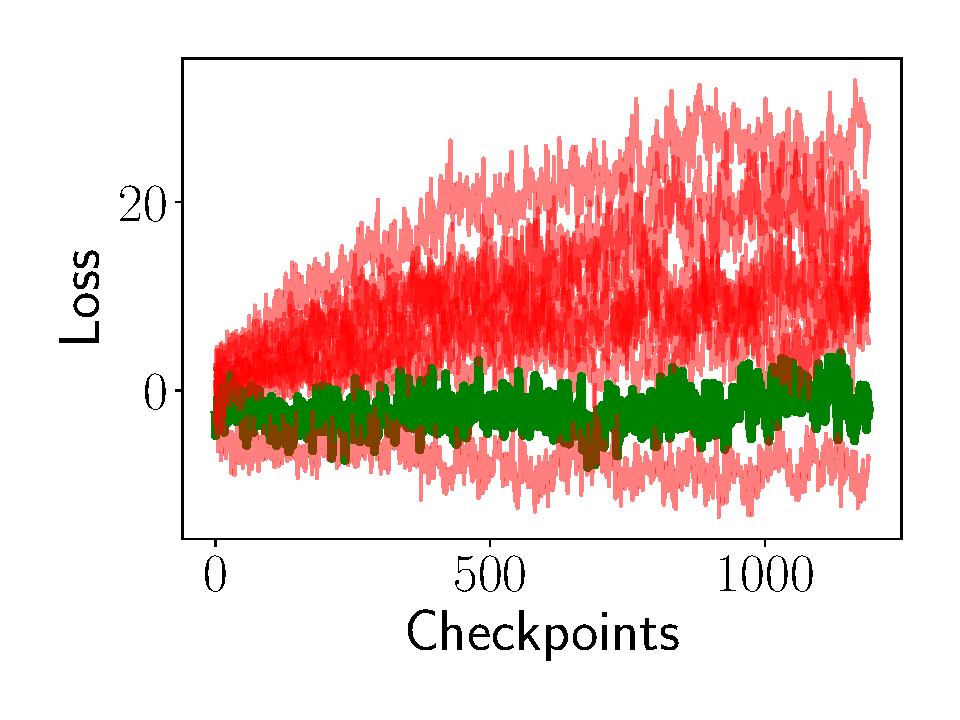
\includegraphics[width=\linewidth]{figs/sptd/svhn/losses_id_23.pdf}
%  \end{subfigure}
%  \hfill
%  \begin{subfigure}{.24 \linewidth}
%    \centering
%    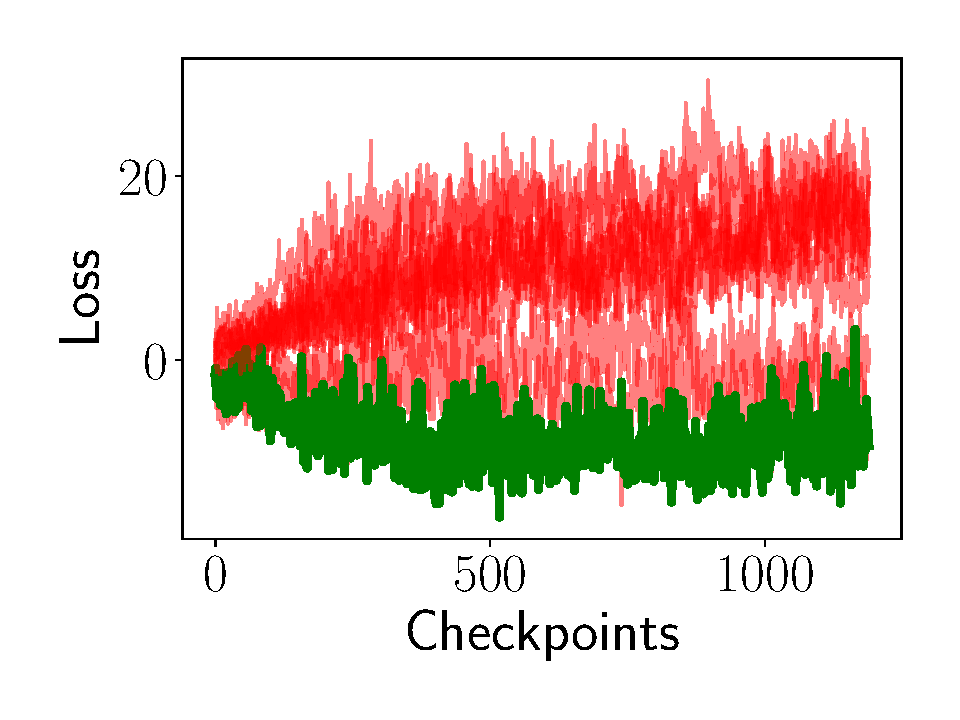
\includegraphics[width=\linewidth]{figs/sptd/svhn/losses_id_32.pdf}
%  \end{subfigure}
% \caption{\textbf{Individual SVHN examples}. We extend Figure~\ref{fig:svhn} by also including the evolution of the confidence, the gap, and the entropy over the course of training in the third row. In the final row, we further plot the loss evolution for all candidate classes. We note that the first two examples are easy to classify as indicated by mostly stationary metrics and a clear loss separation, while the last two examples are harder to classify since they exhibit highly erratic metrics and ambiguous loss curves.}
% % 
% \label{fig:svhn_ext}
% \end{figure}

% \begin{figure}[t]
% \begin{subfigure}{.24 \linewidth}
%   \centering
%   \includegraphics[width=\linewidth]{figs/sptd/gtsrb/data_id_64.pdf}
% \end{subfigure}
% \hfill
% \begin{subfigure}{.24 \linewidth}
%   \centering
%   \includegraphics[width=\linewidth]{figs/sptd/gtsrb/data_id_0.pdf}
% \end{subfigure}
% \hfill
% \begin{subfigure}{.24 \linewidth}
%   \centering
%   \includegraphics[width=\linewidth]{figs/sptd/gtsrb/data_id_3.pdf}
% \end{subfigure}
% \hfill
% \begin{subfigure}{.24 \linewidth}
%   \centering
%   \includegraphics[width=\linewidth]{figs/sptd/gtsrb/data_id_66.pdf}
% \end{subfigure}

% \begin{subfigure}{.24 \linewidth}
%   \centering
%   \includegraphics[width=\linewidth]{figs/sptd/gtsrb/metrics_id_64.pdf}
% \end{subfigure}
% \hfill
% \begin{subfigure}{.24 \linewidth}
%   \centering
%   \includegraphics[width=\linewidth]{figs/sptd/gtsrb/metrics_id_0.pdf}
% \end{subfigure}
% \hfill
% \begin{subfigure}{.24 \linewidth}
%   \centering
%   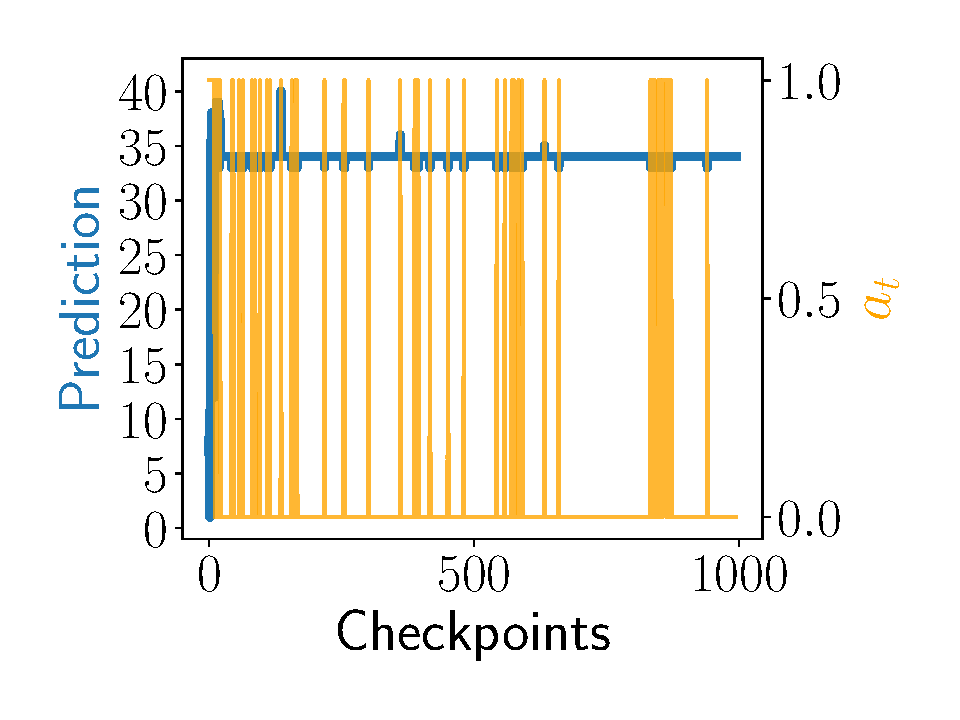
\includegraphics[width=\linewidth]{figs/sptd/gtsrb/metrics_id_3.pdf}
% \end{subfigure}
% \hfill
% \begin{subfigure}{.24 \linewidth}
%   \centering
%   \includegraphics[width=\linewidth]{figs/sptd/gtsrb/metrics_id_66.pdf}
% \end{subfigure}

%  \begin{subfigure}{.24 \linewidth}
%    \centering
%    \includegraphics[width=\linewidth]{figs/sptd/gtsrb/metrics_alt_id_leg_64.pdf}
%  \end{subfigure}
%  \hfill
%  \begin{subfigure}{.24 \linewidth}
%    \centering
%    \includegraphics[width=\linewidth]{figs/sptd/gtsrb/metrics_alt_id_0.pdf}
%  \end{subfigure}
%  \hfill
%  \begin{subfigure}{.24 \linewidth}
%    \centering
%    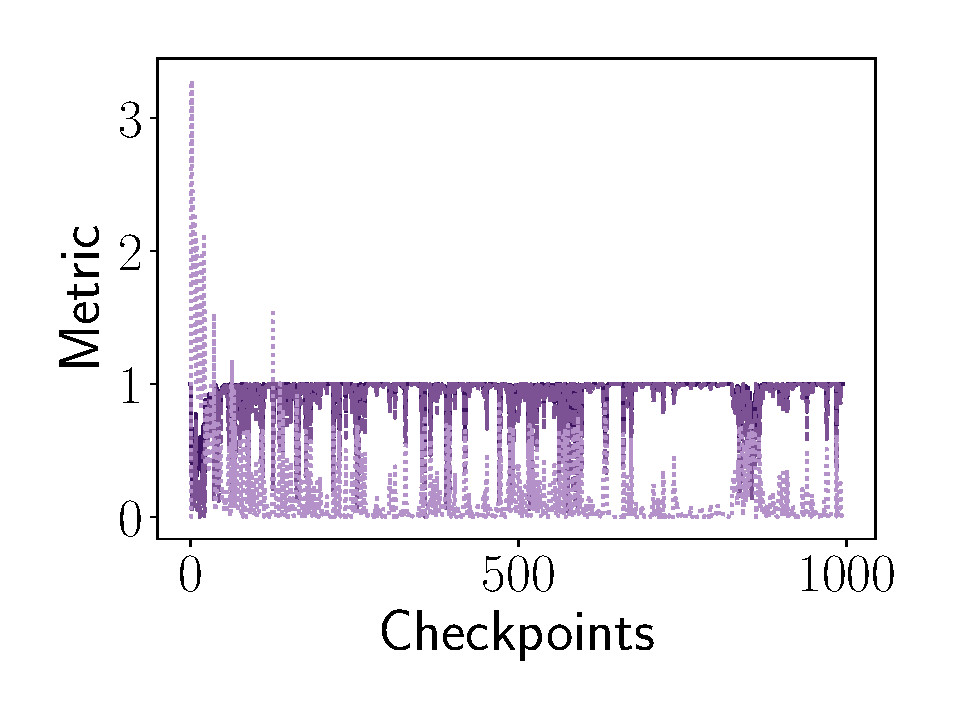
\includegraphics[width=\linewidth]{figs/sptd/gtsrb/metrics_alt_id_3.pdf}
%  \end{subfigure}
%  \hfill
%  \begin{subfigure}{.24 \linewidth}
%    \centering
%    \includegraphics[width=\linewidth]{figs/sptd/gtsrb/metrics_alt_id_66.pdf}
%  \end{subfigure}

%  \begin{subfigure}{.24 \linewidth}
%    \centering
%    \includegraphics[width=\linewidth]{figs/sptd/gtsrb/losses_id_leg_64.pdf}
%  \end{subfigure}
%  \hfill
%  \begin{subfigure}{.24 \linewidth}
%    \centering
%    \includegraphics[width=\linewidth]{figs/sptd/gtsrb/losses_id_0.pdf}
%  \end{subfigure}
%  \hfill
%  \begin{subfigure}{.24 \linewidth}
%    \centering
%    \includegraphics[width=\linewidth]{figs/sptd/gtsrb/losses_id_3.pdf}
%  \end{subfigure}
%  \hfill
%  \begin{subfigure}{.24 \linewidth}
%    \centering
%    \includegraphics[width=\linewidth]{figs/sptd/gtsrb/losses_id_66.pdf}
%  \end{subfigure}
% \caption{\textbf{Individual GTSRB examples}. Similar as Figure~\ref{fig:svhn_ext}.}
% \label{fig:gtsrb}
% \end{figure}


% \begin{figure}[t]
% \begin{subfigure}{.24 \linewidth}
%   \centering
%   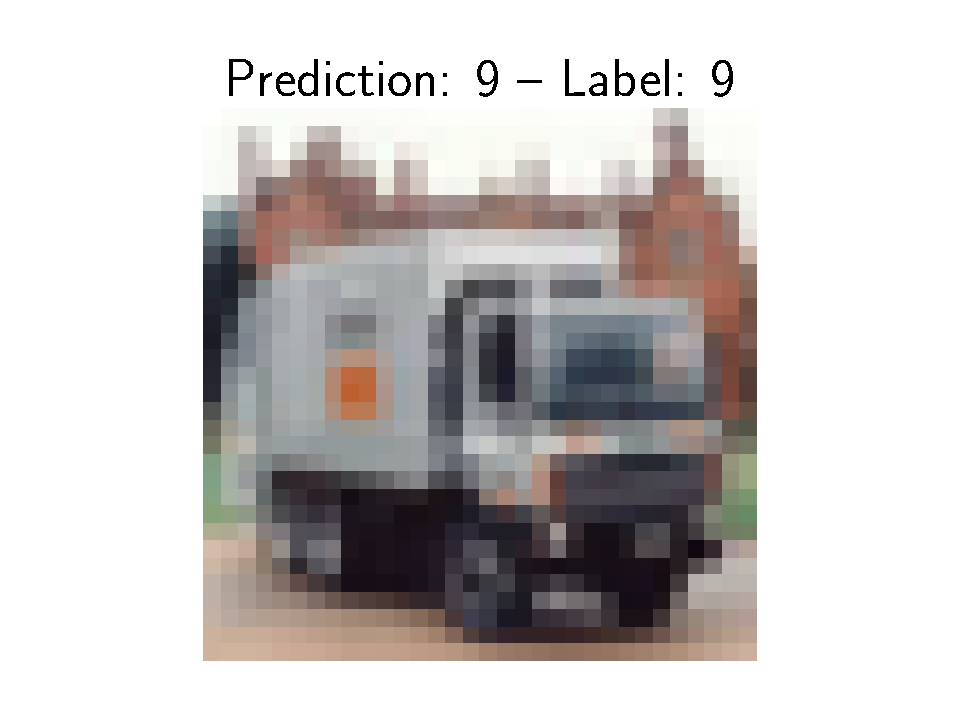
\includegraphics[width=\linewidth]{figs/sptd/cifar10/data_id_11.pdf}
% \end{subfigure}
% \hfill
% \begin{subfigure}{.24 \linewidth}
%   \centering
%   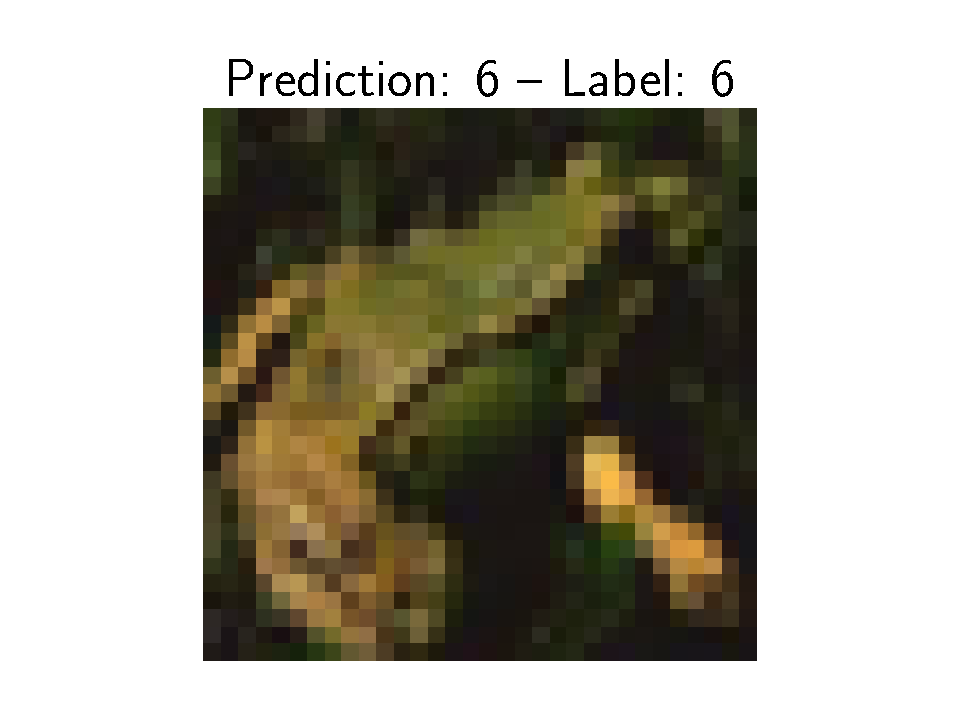
\includegraphics[width=\linewidth]{figs/sptd/cifar10/data_id_41.pdf}
% \end{subfigure}
% \hfill
% \begin{subfigure}{.24 \linewidth}
%   \centering
%   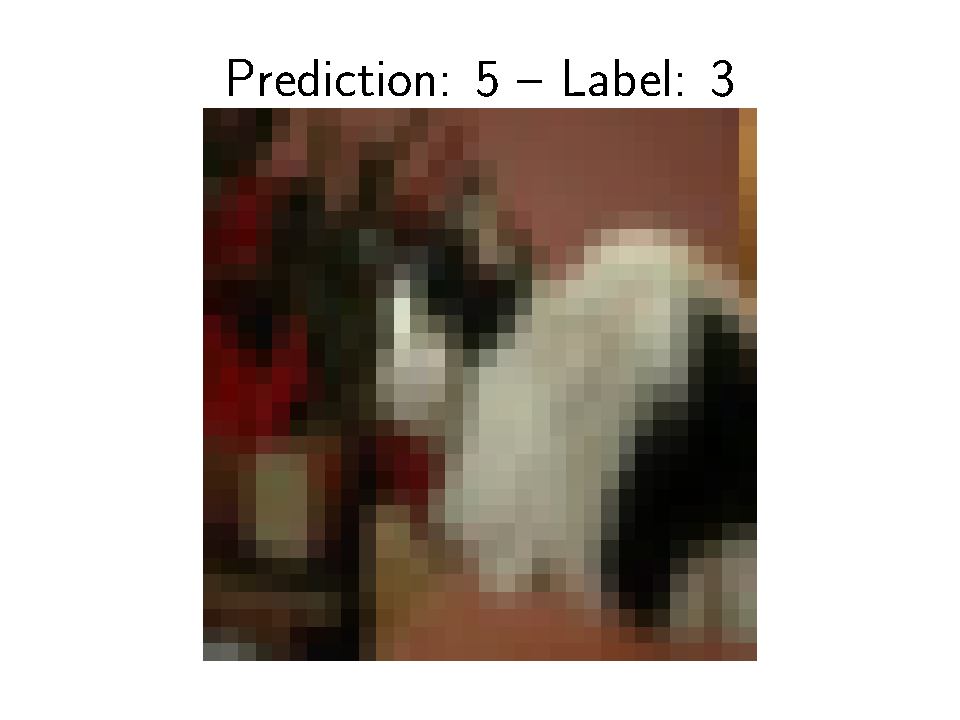
\includegraphics[width=\linewidth]{figs/sptd/cifar10/data_id_78.pdf}
% \end{subfigure}
% \hfill
% \begin{subfigure}{.24 \linewidth}
%   \centering
%   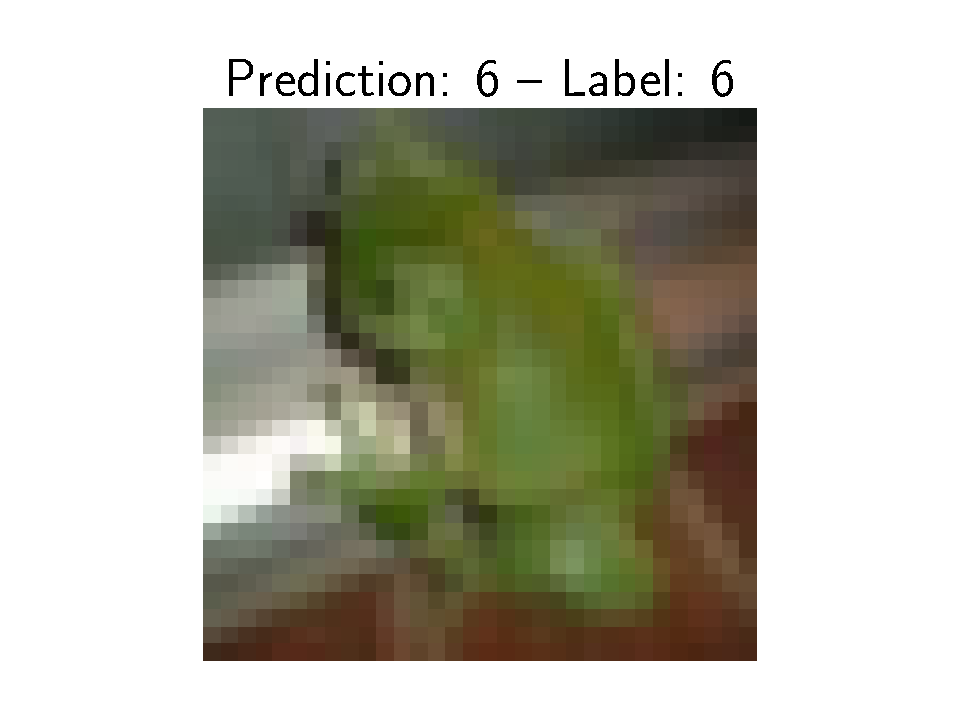
\includegraphics[width=\linewidth]{figs/sptd/cifar10/data_id_7.pdf}
% \end{subfigure}

% \begin{subfigure}{.24 \linewidth}
%   \centering
%   \includegraphics[width=\linewidth]{figs/sptd/cifar10/metrics_id_11.pdf}
% \end{subfigure}
% \hfill
% \begin{subfigure}{.24 \linewidth}
%   \centering
%   \includegraphics[width=\linewidth]{figs/sptd/cifar10/metrics_id_41.pdf}
% \end{subfigure}
% \hfill
% \begin{subfigure}{.24 \linewidth}
%   \centering
%   \includegraphics[width=\linewidth]{figs/sptd/cifar10/metrics_id_78.pdf}
% \end{subfigure}
% \hfill
% \begin{subfigure}{.24 \linewidth}
%   \centering
%   \includegraphics[width=\linewidth]{figs/sptd/cifar10/metrics_id_7.pdf}
% \end{subfigure}

%  \begin{subfigure}{.24 \linewidth}
%    \centering
%    \includegraphics[width=\linewidth]{figs/sptd/cifar10/metrics_alt_id_leg_11.pdf}
%  \end{subfigure}
%  \hfill
%  \begin{subfigure}{.24 \linewidth}
%    \centering
%    \includegraphics[width=\linewidth]{figs/sptd/cifar10/metrics_alt_id_41.pdf}
%  \end{subfigure}
%  \hfill
%  \begin{subfigure}{.24 \linewidth}
%    \centering
%    \includegraphics[width=\linewidth]{figs/sptd/cifar10/metrics_alt_id_78.pdf}
%  \end{subfigure}
%  \hfill
%  \begin{subfigure}{.24 \linewidth}
%    \centering
%    \includegraphics[width=\linewidth]{figs/sptd/cifar10/metrics_alt_id_7.pdf}
%  \end{subfigure}

%  \begin{subfigure}{.24 \linewidth}
%    \centering
%    \includegraphics[width=\linewidth]{figs/sptd/cifar10/losses_id_leg_11.pdf}
%  \end{subfigure}
%  \hfill
%  \begin{subfigure}{.24 \linewidth}
%    \centering
%    \includegraphics[width=\linewidth]{figs/sptd/cifar10/losses_id_41.pdf}
%  \end{subfigure}
%  \hfill
%  \begin{subfigure}{.24 \linewidth}
%    \centering
%    \includegraphics[width=\linewidth]{figs/sptd/cifar10/losses_id_78.pdf}
%  \end{subfigure}
%  \hfill
%  \begin{subfigure}{.24 \linewidth}
%    \centering
%    \includegraphics[width=\linewidth]{figs/sptd/cifar10/losses_id_7.pdf}
%  \end{subfigure}
% \caption{\textbf{Individual CIFAR-10 examples}. Similar as Figure~\ref{fig:svhn_ext}.}
% \label{fig:cifar10}
% \end{figure}

% \begin{figure}[t]
% \begin{subfigure}{.24 \linewidth}
%   \centering
%   \includegraphics[width=\linewidth]{figs/sptd/cifar100/data_id_44.pdf}
% \end{subfigure}
% \hfill
% \begin{subfigure}{.24 \linewidth}
%   \centering
%   \includegraphics[width=\linewidth]{figs/sptd/cifar100/data_id_13.pdf}
% \end{subfigure}
% \hfill
% \begin{subfigure}{.24 \linewidth}
%   \centering
%   \includegraphics[width=\linewidth]{figs/sptd/cifar100/data_id_99.pdf}
% \end{subfigure}
% \hfill
% \begin{subfigure}{.24 \linewidth}
%   \centering
%   \includegraphics[width=\linewidth]{figs/sptd/cifar100/data_id_92.pdf}
% \end{subfigure}

% \begin{subfigure}{.24 \linewidth}
%   \centering
%   \includegraphics[width=\linewidth]{figs/sptd/cifar100/metrics_id_44.pdf}
% \end{subfigure}
% \hfill
% \begin{subfigure}{.24 \linewidth}
%   \centering
%   \includegraphics[width=\linewidth]{figs/sptd/cifar100/metrics_id_13.pdf}
% \end{subfigure}
% \hfill
% \begin{subfigure}{.24 \linewidth}
%   \centering
%   \includegraphics[width=\linewidth]{figs/sptd/cifar100/metrics_id_99.pdf}
% \end{subfigure}
% \hfill
% \begin{subfigure}{.24 \linewidth}
%   \centering
%   \includegraphics[width=\linewidth]{figs/sptd/cifar100/metrics_id_92.pdf}
% \end{subfigure}

%  \begin{subfigure}{.24 \linewidth}
%    \centering
%    \includegraphics[width=\linewidth]{figs/sptd/cifar100/metrics_alt_id_leg_44.pdf}
%  \end{subfigure}
%  \hfill
%  \begin{subfigure}{.24 \linewidth}
%    \centering
%    \includegraphics[width=\linewidth]{figs/sptd/cifar100/metrics_alt_id_13.pdf}
%  \end{subfigure}
%  \hfill
%  \begin{subfigure}{.24 \linewidth}
%    \centering
%    \includegraphics[width=\linewidth]{figs/sptd/cifar100/metrics_alt_id_99.pdf}
%  \end{subfigure}
%  \hfill
%  \begin{subfigure}{.24 \linewidth}
%    \centering
%    \includegraphics[width=\linewidth]{figs/sptd/cifar100/metrics_alt_id_92.pdf}
%  \end{subfigure}

%  \begin{subfigure}{.24 \linewidth}
%    \centering
%    \includegraphics[width=\linewidth]{figs/sptd/cifar100/losses_id_leg_44.pdf}
%  \end{subfigure}
%  \hfill
%  \begin{subfigure}{.24 \linewidth}
%    \centering
%    \includegraphics[width=\linewidth]{figs/sptd/cifar100/losses_id_13.pdf}
%  \end{subfigure}
%  \hfill
%  \begin{subfigure}{.24 \linewidth}
%    \centering
%    \includegraphics[width=\linewidth]{figs/sptd/cifar100/losses_id_99.pdf}
%  \end{subfigure}
%  \hfill
%  \begin{subfigure}{.24 \linewidth}
%    \centering
%    \includegraphics[width=\linewidth]{figs/sptd/cifar100/losses_id_92.pdf}
%  \end{subfigure}
% \caption{\textbf{Individual CIFAR-100 examples}. Similar as Figure~\ref{fig:svhn_ext}.}
% \label{fig:cifar100}
% \end{figure}

% \begin{figure}[t]
% \begin{subfigure}{.24 \linewidth}
%   \centering
%   \includegraphics[width=\linewidth]{figs/sptd/catsdogs/data_id_85.pdf}
% \end{subfigure}
% \hfill
% \begin{subfigure}{.24 \linewidth}
%   \centering
%   \includegraphics[width=\linewidth]{figs/sptd/catsdogs/data_id_3087.pdf}
% \end{subfigure}
% \hfill
% \begin{subfigure}{.24 \linewidth}
%   \centering
%   \includegraphics[width=\linewidth]{figs/sptd/catsdogs/data_id_3080.pdf}
% \end{subfigure}
% \hfill
% \begin{subfigure}{.24 \linewidth}
%   \centering
%   \includegraphics[width=\linewidth]{figs/sptd/catsdogs/data_id_58.pdf}
% \end{subfigure}

% \begin{subfigure}{.24 \linewidth}
%   \centering
%   \includegraphics[width=\linewidth]{figs/sptd/catsdogs/metrics_id_85.pdf}
% \end{subfigure}
% \hfill
% \begin{subfigure}{.24 \linewidth}
%   \centering
%   \includegraphics[width=\linewidth]{figs/sptd/catsdogs/metrics_id_3087.pdf}
% \end{subfigure}
% \hfill
% \begin{subfigure}{.24 \linewidth}
%   \centering
%   \includegraphics[width=\linewidth]{figs/sptd/catsdogs/metrics_id_3080.pdf}
% \end{subfigure}
% \hfill
% \begin{subfigure}{.24 \linewidth}
%   \centering
%   \includegraphics[width=\linewidth]{figs/sptd/catsdogs/metrics_id_58.pdf}
% \end{subfigure}

%  \begin{subfigure}{.24 \linewidth}
%    \centering
%    \includegraphics[width=\linewidth]{figs/sptd/catsdogs/metrics_alt_id_leg_85.pdf}
%  \end{subfigure}
%  \hfill
%  \begin{subfigure}{.24 \linewidth}
%    \centering
%    \includegraphics[width=\linewidth]{figs/sptd/catsdogs/metrics_alt_id_3087.pdf}
%  \end{subfigure}
%  \hfill
%  \begin{subfigure}{.24 \linewidth}
%    \centering
%    \includegraphics[width=\linewidth]{figs/sptd/catsdogs/metrics_alt_id_3080.pdf}
%  \end{subfigure}
%  \hfill
%  \begin{subfigure}{.24 \linewidth}
%    \centering
%    \includegraphics[width=\linewidth]{figs/sptd/catsdogs/metrics_alt_id_58.pdf}
%  \end{subfigure}

%  \begin{subfigure}{.24 \linewidth}
%    \centering
%    \includegraphics[width=\linewidth]{figs/sptd/catsdogs/losses_id_leg_85.pdf}
%  \end{subfigure}
%  \hfill
%  \begin{subfigure}{.24 \linewidth}
%    \centering
%    \includegraphics[width=\linewidth]{figs/sptd/catsdogs/losses_id_3087.pdf}
%  \end{subfigure}
%  \hfill
%  \begin{subfigure}{.24 \linewidth}
%    \centering
%    \includegraphics[width=\linewidth]{figs/sptd/catsdogs/losses_id_3080.pdf}
%  \end{subfigure}
%  \hfill
%  \begin{subfigure}{.24 \linewidth}
%    \centering
%    \includegraphics[width=\linewidth]{figs/sptd/catsdogs/losses_id_58.pdf}
%  \end{subfigure}
% \caption{\textbf{Individual Cats \& Dogs examples}. Similar as Figure~\ref{fig:svhn_ext}.}
% \label{fig:catsdogs}
% \end{figure}

% \begin{figure}[ht]
% \begin{subfigure}{.24 \linewidth}
%   \centering
%   \includegraphics[width=\linewidth]{figs/sptd/cifar10_metr_et_leg.pdf}
% \end{subfigure}
% \hfill
% \begin{subfigure}{.24 \linewidth}
%   \centering
%   \includegraphics[width=\linewidth]{figs/sptd/svhn_metr_et.pdf}
% \end{subfigure}
% \hfill
% \begin{subfigure}{.24 \linewidth}
%   \centering
%   \includegraphics[width=\linewidth]{figs/sptd/gtsrb_metr_et.pdf}
% \end{subfigure}
% \hfill
% \begin{subfigure}{.24 \linewidth}
%   \centering
%   \includegraphics[width=\linewidth]{figs/sptd/cifar100_metr_et.pdf}
% \end{subfigure}

% \begin{subfigure}{.24 \linewidth}
%   \centering
%   \includegraphics[width=\linewidth]{figs/sptd/cifar10_metr_et_smooth_leg.pdf}
%   \caption{CIFAR-10}
% \end{subfigure}
% \hfill
% \begin{subfigure}{.24 \linewidth}
%   \centering
%   \includegraphics[width=\linewidth]{figs/sptd/svhn_metr_et_smooth.pdf}
%   \caption{SVHN}
% \end{subfigure}
% \hfill
% \begin{subfigure}{.24 \linewidth}
%   \centering
%   \includegraphics[width=\linewidth]{figs/sptd/gtsrb_metr_et_smooth.pdf}
%   \caption{GTSRB}
% \end{subfigure}
% \hfill
% \begin{subfigure}{.24 \linewidth}
%   \centering
%   \includegraphics[width=\linewidth]{figs/sptd/cifar100_metr_et_smooth.pdf}
%   \caption{CIFAR-100}
% \end{subfigure}
% \caption{\textbf{Coverage/error trade-off when incorporating $e_t$ into \smin and \savg}. In the first row, the solid blue line corresponds to \texttt{NNTD}$(s_\text{avg}, 0.05)$ while the dashed lines show the performance when we incorporate an empirical estimate of $e_t$ for various weightings $v_i$. In the second row, maintaining the solid blue line as \texttt{NNTD}$(s_\text{avg}, 0.05)$, we fix $v_t$ at $k=0.05$ and test various continuous approximations of $e_t$ as $e_t = 1 - t^k$ for $k \in (0,1]$. Overall, we find that introducing an adaptable $e_t$ does not further improve the performance of \smin and \savg with $e_t = 0$.}
% \label{fig:et_incorp}
% \end{figure}

% \begin{figure}[ht]
% \begin{subfigure}{.24 \linewidth}
%   \centering
%   \includegraphics[width=\linewidth]{figs/sptd/cifar10_metr_cont_leg.pdf}
%   \caption{CIFAR-10}
% \end{subfigure}
% \hfill
% \begin{subfigure}{.24 \linewidth}
%   \centering
%   \includegraphics[width=\linewidth]{figs/sptd/svhn_metr_cont.pdf}
%   \caption{SVHN}
% \end{subfigure}
% \hfill
% \begin{subfigure}{.24 \linewidth}
%   \centering
%   \includegraphics[width=\linewidth]{figs/sptd/gtsrb_metr_cont.pdf}
%   \caption{GTSRB}
% \end{subfigure}
% \hfill
% \begin{subfigure}{.24 \linewidth}
%   \centering
%   \includegraphics[width=\linewidth]{figs/sptd/cifar100_metr_cont.pdf}
%   \caption{CIFAR-100}
% \end{subfigure}
% \caption{\textbf{Coverage/error trade-off of \nntd for alternate scores}. We find that neither the jump score, nor any of the weighted variance metrics at their optimal $k$ for $v_i$ outperform \texttt{NNTD}$(s_\text{avg}, 0.05)$.}
% \label{fig:scores_alt}
% \end{figure}

% \begin{figure}[t]
% \begin{subfigure}{.24 \linewidth}
%   \centering
%   \includegraphics[width=\linewidth]{figs/sptd/weightings_conc.pdf}
%   \caption{Concave weighting}
% \end{subfigure}
% \hfill
% \begin{subfigure}{.24 \linewidth}
%   \centering
%   \includegraphics[width=\linewidth]{figs/sptd/cifar10/cifar10_pred_k_conc.pdf}
%   \caption{CIFAR-10}
% \end{subfigure}
% \hfill
% \begin{subfigure}{.24 \linewidth}
%   \centering
%   \includegraphics[width=\linewidth]{figs/sptd/svhn/svhn_pred_k_conc.pdf}
%   \caption{SVHN}
% \end{subfigure}
% \hfill
% \begin{subfigure}{.24 \linewidth}
%   \centering
%   \includegraphics[width=\linewidth]{figs/sptd/gtsrb/gtsrb_pred_k_conc.pdf}
%   \caption{GTSRB}
% \end{subfigure}
% \caption{\textbf{Concave weighting used in $v_t = 1 - t^k$}. Overall, since the best concave weighting is given by $k=1$, we conclude that no concave weighting outperforms any convex weighting.}
% \label{fig:conc_weighting}
% \end{figure}

% \begin{table*}[t]
% \scriptsize
% \tabcolsep=0.15cm
%     \centering {
%         \caption{\textbf{Coverage/Error trade-off of \nntd as a function of the accounted data points (CIFAR-10 left, SVHN right)}. We observe that large parts of the training process contain valuable sigals for selective classification.}
%     \label{tab:perc_checkp}
%     \vspace{10pt}
%      \begin{tabular}{ c c c c c c c} 
%     \toprule
%     Target Coverage & 100\% & 90\% &  80\% & 50\% &  20\% & 10\% \\  
%      \midrule
%         100\% & 6.07 & 6.08 & 6.10 & 6.15 & 6.18 & 6.20 \\
%         95\% & 3.24 & 3.25 & 3.25 & 3.31 & 3.34 & 3.39 \\
%         90\% & 1.83 & 1.83 & 1.84 & 1.88 & 1.91 & 1.93 \\
%         80\% & 0.64 & 0.65 & 0.67 & 0.72 & 0.78 & 0.79 \\
%         70\% & 0.34 & 0.34 & 0.36 & 0.38 & 0.40 & 0.40 \\
%     \bottomrule
%     \end{tabular}
%     \qquad
%     \begin{tabular}{ c c c c c c c} 
%     \toprule
%     Target Coverage & 100\% & 90\% &  80\% & 50\% &  20\% & 10\% \\  
%      \midrule
%         100\% & 2.68 & 2.70 & 2.73 & 2.83 & 2.88 & 2.92 \\
%         95\% & 0.88 & 0.90 & 0.93 & 1.01 & 1.09 & 1.11\\
%         90\% & 0.55 & 0.57 & 0.59 & 0.62 & 0.68 & 0.73\\
%         80\% & 0.38 & 0.39 & 0.40 & 0.45 & 0.51 & 0.53\\
%         70\% & 0.33 & 0.33 & 0.35 & 0.41 & 0.44 & 0.45\\
%     \bottomrule
%     \end{tabular}
%     }

% \end{table*} 

% \begin{table*}[t]
% \small
% \tabcolsep=0.13cm
%     \centering {
%         \caption{\textbf{ImageNet coverage/error results}. We observe that \nntd outperforms the \sr baseline by a large margin and offers comparable performance as \sat.}
%     \label{tab:imagenet}
%     \vspace{10pt}
%      \begin{tabular}{ c  c c c c  c c} 
%     \toprule
%     Target & \multicolumn{2}{c}{\nntd} & \multicolumn{2}{c}{\sat} & \multicolumn{2}{c}{\sr}  \\ 
%      \cmidrule(lr){2-3} \cmidrule(lr){4-5} \cmidrule(lr){6-7} 
%     Error & Cov $\uparrow$ & Err & Cov $\uparrow$ & Err & Cov $\uparrow$ & Err \\  
%      \midrule
%         10\% & \textbf{54.4} & 10.0 & 53.7 & 10.0 & 15.2 & 10.0 \\
%         5\% & \textbf{26.3} & 5.0 & 25.8 & 5.0 & 5.4 & 5.0 \\
%         2\% & 8.1 & 2.0 & \textbf{8.8} & 2.0 & 1.1 & 2.0 \\
%         1\% & 3.6 & 1.0 & \textbf{4.0} & 1.8 & 0.7 & 1.8\\
%         0.5\% & \textbf{2.3} & 0.7 & 2.2 & 0.6 & 0.0 & 0.0 \\
%     \bottomrule
%     \end{tabular}
%     \qquad
%     \begin{tabular}{ c  c c c c  c c} 
%     \toprule
%     Target & \multicolumn{2}{c}{\nntd}  & \multicolumn{2}{c}{\sat} & \multicolumn{2}{c}{\sr}  \\ 
%      \cmidrule(lr){2-3} \cmidrule(lr){4-5} \cmidrule(lr){6-7} 
%     Coverage & Cov & Err $\downarrow$ & Cov & Err $\downarrow$ & Cov & Err $\downarrow$ \\  
%      \midrule
%         100\% & 100 & \textbf{24.2} & 100 & \textbf{24.2} & 100 & \textbf{24.2} \\
%         95\% & 95.0 & 23.2 & 95.0 & \textbf{22.8} & 95.0 & 23.5 \\
%         90\% & 90.0 & \textbf{22.5} & 90.0 & 22.6 & 90.0 & 22.9 \\
%         80\% & 80.0 & \textbf{18.0} & 80.0 & 18.4 & 80.0 & 21.7 \\
%         70\% & 70.0 & \textbf{14.1} & 70.0 & 14.3 & 70.0 & 20.7 \\
%     \bottomrule
%     \end{tabular}
%     }
% \end{table*} 

% \begin{table*}[t]
% \small
% \tabcolsep=0.13cm
%     \centering {
%         \caption{\textbf{Performance of \nntd in comparison with OOD scores}. We find that \nntd significantly outperforms common OOD detection approaches for the purpose of selective classification.}
%     \label{tab:ood}
%     \vspace{10pt}
%      \begin{tabular}{ c c  c c  c c  c c  c c} 
%     \toprule
%      \multirow{2}{*}{Dataset} & Target & \multicolumn{2}{c}{\nntd} & \multicolumn{2}{c}{\texttt{Energy}}   & \multicolumn{2}{c}{\texttt{Mahalanobis}} & \multicolumn{2}{c}{\texttt{ODIN}} \\ 
%      \cmidrule(lr){3-4} \cmidrule(lr){5-6} \cmidrule(lr){7-8} \cmidrule(lr){9-10}
%       & Coverage & Cov & Err $\downarrow$ & Cov & Err $\downarrow$  & Cov & Err $\downarrow$ & Cov & Err $\downarrow$ \\  
%      \midrule
%      \multirow{5}{*}{CIFAR-10}     
%         & 100\% & 100 & \textbf{6.07} & 100 & \textbf{6.07} & 100 & \textbf{6.07} & 100 & \textbf{6.07} \\
%         & 95\% & 95.0 & \textbf{3.24} & 95.0 & 3.99 & 95.0 & 4.44 & 95.1 & 6.04  \\
%         & 90\% & 90.1 & \textbf{1.83} & 90.0 & 2.67 & 90.0 & 2.93 & 88.9 & 6.01 \\
%         & 80\% & 79.9 & \textbf{0.64} & 80.0 & 1.10 & 80.1 & 1.20 & 88.9 & 6.01 \\
%         & 70\% & 69.8 & \textbf{0.34} & 70.0 & 0.83 & 69.9 & 0.82 & 68.3 & 4.41  \\
%      \midrule
%      \multirow{5}{*}{SVHN}     
%         & 100\% & 100 & \textbf{2.68} & 100 & \textbf{2.68} & 100 & \textbf{2.68} & 100 & \textbf{2.68}  \\
%         & 95\% & 95.0 & \textbf{0.88} & 95.1 & 1.35 & 95.1 & 1.51 & 95.0 & 2.67  \\
%         & 90\% & 90.1 & \textbf{0.55} & 89.9 & 0.92 & 90.0 & 1.04 & 89.9 & 2.64 \\
%         & 80\% & 79.9 & \textbf{0.38} & 79.9 & 0.70 & 80.3 & 0.70 & 81.9 & 2.51  \\
%         & 70\% & 69.8 & \textbf{0.33} & 70.0 & 0.58 & 69.8 & 0.58 & 74.9 & 2.18  \\
%     \bottomrule
%     \end{tabular}}
% \end{table*}

% \begin{sidewaystable}
% \tiny
% \tabcolsep=0.1cm
%     \centering {
%         \caption{\textbf{Performance at low target errors}. Same results as in Table~\ref{tab:target_acc} but includes standard deviations.
%     }
%     \label{tab:target_acc_ext}
%      \begin{tabular}{ c c c c c c  c c  c c  c c c c } 
%      \toprule
%      \multirow{2}{*}{Dataset} & {Target} & \multicolumn{2}{c}{\nntd} & \multicolumn{2}{c}{\sat}   & \multicolumn{2}{c}{\dg} & \multicolumn{2}{c}{\sn}  & \multicolumn{2}{c}{\sr} & \multicolumn{2}{c}{\mcdo} \\ 
%      \cmidrule(lr){3-4} \cmidrule(lr){5-6} \cmidrule(lr){7-8} \cmidrule(lr){9-10} \cmidrule(lr){11-12} \cmidrule(lr){13-14}
%       & Error & Cov $\uparrow$ & Err & Cov $\uparrow$ & Err  & Cov $\uparrow$ & Err & Cov $\uparrow$ & Err & Cov $\uparrow$ & Err & Cov $\uparrow$ & Err \\ 
%      \midrule
%     \multirow{3}{*}{CIFAR-10}       & 2\%  & \textbf{91.2} ($\pm$ 0.05) & 1.99 ($\pm$ 0.01) & 90.3 ($\pm$ 0.03)  & 1.97 ($\pm$ 0.02)  & 89.1 ($\pm$ 0.04)  & 2.02 ($\pm$ 0.01) & 88.3 ($\pm$ 0.03) & 2.03 ($\pm$ 0.02) & 85.8 ($\pm$ 0.08) & 1.98 ($\pm$ 0.02) & 86.1 ($\pm$ 0.07) & 2.01 ($\pm$ 0.01) \\
%                     & 1\%  & \textbf{86.4} ($\pm$ 0.03) & 1.00 ($\pm$ 0.01) & \textbf{86.1} ($\pm$ 0.02) & 1.02 ($\pm$ 0.02)  & 85.5 ($\pm$ 0.07) & 1.03 ($\pm$ 0.02) & 84.4 ($\pm$ 0.06) & 0.98 ($\pm$ 0.02)  & 79.1 ($\pm$ 0.08) & 1.01 ($\pm$ 0.03)  & 79.9 ($\pm$ 0.08) & 1.01 ($\pm$ 0.03) \\
%                     & 0.5\%  & \textbf{75.9} ($\pm$ 0.04)  & 0.49 ($\pm$ 0.02)  & \textbf{76.0} ($\pm$ 0.05) & 0.51 ($\pm$ 0.02)  & 75.2 ($\pm$ 0.08) & 0.5 ($\pm$ 0.03) & 74.7 ($\pm$ 0.09) & 0.49 ($\pm$ 0.01) & 71.2 ($\pm$ 0.05) & 0.51 ($\pm$ 0.02) & 72.0 ($\pm$ 0.03) & 0.50 ($\pm$ 0.03) \\
%     \midrule
%     \multirow{3}{*}{SVHN}      & 2\%  & \textbf{98.5} ($\pm$ 0.05) & 1.98 ($\pm$ 0.03) & \textbf{98.2} ($\pm$ 0.04) & 1.99 ($\pm$ 0.02) & 97.8 ($\pm$ 0.03) & 2.06 ($\pm$ 0.05) & 97.7 ($\pm$ 0.06) & 2.03 ($\pm$ 0.02) & 97.6 ($\pm$ 0.05) & 1.99 ($\pm$ 0.03) & 97.9 ($\pm$ 0.03) & 2.00 ($\pm$ 0.04) \\
%                     & 1\%  & \textbf{96.3} ($\pm$ 0.03)  & 0.99 ($\pm$ 0.02) & 95.7 ($\pm$ 0.02) & 1.03 ($\pm$ 0.03) & 94.8 ($\pm$ 0.04) & 0.99 ($\pm$ 0.01) & 94.5 ($\pm$ 0.03) & 1.04 ($\pm$ 0.02) & 93.5 ($\pm$ 0.05) & 1.01 ($\pm$ 0.03) & 94.1 ($\pm$ 0.06) & 0.97 ($\pm$ 0.02) \\
%                     & 0.5\%  & \textbf{88.1} ($\pm$ 0.02) & 0.50 ($\pm$ 0.02) & \textbf{87.9} ($\pm$ 0.05) & 0.51 ($\pm$ 0.01) & 86.4 ($\pm$ 0.04) & 0.51 ($\pm$ 0.01) & 86.0 ($\pm$ 0.04) & 0.51 ($\pm$ 0.01) & 70.0 ($\pm$ 0.09) & 0.50 ($\pm$ 0.04) & 70.1 ($\pm$ 0.04) & 0.49 ($\pm$ 0.03) \\
%     \midrule
%      \multirow{3}{*}{Cats \& Dogs}  & 2\%  & 97.7 ($\pm$ 0.09) & 2.01 ($\pm$ 0.03) & \textbf{98.2} ($\pm$ 0.02) & 1.98 ($\pm$ 0.03) & \textbf{98.0} ($\pm$ 0.05) & 2.03 ($\pm$ 0.02) & 97.4 ($\pm$ 0.05) & 1.98 ($\pm$ 0.03) & 95.1 ($\pm$ 0.12) & 1.99 ($\pm$ 0.04)  & 95.7 ($\pm$ 0.10) & 1.99 ($\pm$ 0.03) \\ 
%                    & 1\%  & 93.1 ($\pm$ 0.03) & 1.01 ($\pm$ 0.02) & \textbf{93.6} ($\pm$ 0.02) & 0.98 ($\pm$ 0.03) &  92.6 ($\pm$ 0.08) & 0.97 ($\pm$ 0.04) & 92.2 ($\pm$ 0.05) & 0.98 ($\pm$ 0.02) & 86.9 ($\pm$ 0.13) & 0.98 ($\pm$ 0.04) & 88.6 ($\pm$ 0.09) & 1.01 ($\pm$ 0.02) \\ 
%                    & 0.5\% & \textbf{85.7} ($\pm$ 0.06) & 0.51 ($\pm$ 0.02) & \textbf{86.0} ($\pm$ 0.04) & 0.49 ($\pm$ 0.01) & 85.3 ($\pm$ 0.02) & 0.49 ($\pm$ 0.02) & 84.8 ($\pm$ 0.03) & 0.46 ($\pm$ 0.05) & 68.4 ($\pm$ 0.10) &  0.48 ($\pm$ 0.02) & 70.1 ($\pm$ 0.08) & 0.51 ($\pm$ 0.03) \\
%     \bottomrule
%     \end{tabular}}
% \end{sidewaystable} 


% \begin{sidewaystable}
% \tiny
% \tabcolsep=0.1cm
%     \centering {
%         \caption{\textbf{Performance at high target coverage}. Same results as in Table~\ref{tab:target_cov} but includes standard deviations.}
%     \label{tab:target_cov_ext}
%      \begin{tabular}{ c c  c c  c c  c c  c c  c c c c } 
%     \toprule
%      \multirow{2}{*}{Dataset} & Target & \multicolumn{2}{c}{\nntd} & \multicolumn{2}{c}{\sat}   & \multicolumn{2}{c}{\dg} & \multicolumn{2}{c}{\sn}  & \multicolumn{2}{c}{\sr} & \multicolumn{2}{c}{\mcdo} \\ 
%      \cmidrule(lr){3-4} \cmidrule(lr){5-6} \cmidrule(lr){7-8} \cmidrule(lr){9-10} \cmidrule(lr){11-12} \cmidrule(lr){13-14}
%       & Coverage & Cov & Err $\downarrow$ & Cov & Err $\downarrow$  & Cov & Err $\downarrow$ & Cov & Err $\downarrow$ & Cov & Err $\downarrow$ & Cov & Err $\downarrow$ \\  
%      \midrule
%      \multirow{5}{*}{CIFAR-10}     
%         & 100\% & 100 ($\pm$ 0.00) & \textbf{6.07} ($\pm$ 0.05)  & 100 ($\pm$ 0.00) & \textbf{6.06} ($\pm$ 0.03) & 100 ($\pm$ 0.00) & 6.11 ($\pm$ 0.05) & 100 ($\pm$ 0.00) & 6.13 ($\pm$ 0.03) & 100 ($\pm$ 0.00) & \textbf{6.07} ($\pm$ 0.05) & 100 ($\pm$ 0.00) & \textbf{6.07} ($\pm$ 0.05) \\
%         & 95\% & 95.0 ($\pm$ 0.01) & \textbf{3.24} ($\pm$ 0.03) & 95.1 ($\pm$ 0.01) & 3.32 ($\pm$ 0.05) & 95.1 ($\pm$ 0.02) & 3.47 ($\pm$ 0.06) & 95.0 ($\pm$ 0.01) & 4.08 ($\pm$ 0.08) & 94.9 ($\pm$ 0.03) & 4.48 ($\pm$ 0.07) & 95.1 ($\pm$ 0.04) & 4.48 ($\pm$ 0.09) \\
%         & 90\% & 90.1 ($\pm$ 0.02) & \textbf{1.83} ($\pm$ 0.04) & 89.9 ($\pm$ 0.02) & 1.90 ($\pm$ 0.02) & 90.0 ($\pm$ 0.01) & 2.19 ($\pm$ 0.05) & 90.1 ($\pm$ 0.02) & 2.29 ($\pm$ 0.03) & 90.1 ($\pm$ 0.02) & 2.78 ($\pm$ 0.06) & 90.0 ($\pm$ 0.02) & 2.87 ($\pm$ 0.07) \\
%         & 80\% & 79.9 ($\pm$ 0.02) & \textbf{0.64} ($\pm$ 0.03) & 80.0 ($\pm$ 0.00) & \textbf{0.65} ($\pm$ 0.04) & 80.1 ($\pm$ 0.03) & \textbf{0.66} ($\pm$ 0.04) & 80.1 ($\pm$ 0.01) & 0.81 ($\pm$ 0.07) & 79.8 ($\pm$ 0.02) & 1.05 ($\pm$ 0.08) & 79.9 ($\pm$ 0.01) & 1.01 ($\pm$ 0.03) \\
%         & 70\% & 69.8 ($\pm$ 0.03) & \textbf{0.34} ($\pm$ 0.04) & 69.9 ($\pm$ 0.03)& \textbf{0.32} ($\pm$ 0.05) & 69.8 ($\pm$ 0.04) & 0.41 ($\pm$ 0.04) & 70.2 ($\pm$ 0.03) & 0.30 ($\pm$ 0.02) & 70.0 ($\pm$ 0.01) & 0.47 ($\pm$ 0.07) & 70.1 ($\pm$ 0.02) & 0.42 ($\pm$ 0.05) \\
%      \midrule
%      \multirow{5}{*}{SVHN}     
%         & 100\% & 100 ($\pm$ 0.00) & \textbf{2.68} ($\pm$ 0.02) & 100 ($\pm$ 0.00) & \textbf{2.71} ($\pm$ 0.03) & 100 ($\pm$ 0.00) & \textbf{2.72} ($\pm$ 0.05) & 100 ($\pm$ 0.00) & 2.77 ($\pm$ 0.06) & 100 ($\pm$ 0.00) & \textbf{2.68} ($\pm$ 0.02) & 100 ($\pm$ 0.00) & \textbf{2.68} ($\pm$ 0.02) \\
%         & 95\% & 95.0 ($\pm$ 0.01) & \textbf{0.88} ($\pm$ 0.02) & 95.1 ($\pm$ 0.02) & 0.95 ($\pm$ 0.03) & 95.1 ($\pm$ 0.01) & 1.01 ($\pm$ 0.06) & 95.0 ($\pm$ 0.02) & 1.07 ($\pm$ 0.05) & 94.9 ($\pm$ 0.03) & 1.15 ($\pm$ 0.11) & 95.1 ($\pm$ 0.02) & 1.12 ($\pm$ 0.07)  \\
%         & 90\% & 90.1 ($\pm$ 0.02) & \textbf{0.55} ($\pm$ 0.4) & 89.9 ($\pm$ 0.01) & \textbf{0.58} ($\pm$ 0.01) & 90.0 ($\pm$ 0.00) & 0.63 ($\pm$ 0.06) & 90.1 ($\pm$ 0.01) & 0.71 ($\pm$ 0.04) & 90.1 ($\pm$ 0.02) & 0.82 ($\pm$ 0.06) & 90.0 ($\pm$ 0.02) & 0.76 ($\pm$ 0.03) \\
%         & 80\% & 79.9 ($\pm$ 0.01) & \textbf{0.38} ($\pm$ 0.02) & 80.0 ($\pm$ 0.01) & \textbf{0.37} ($\pm$ 0.02) & 80.1 ($\pm$ 0.01) & 0.43 ($\pm$ 0.01) & 80.1 ($\pm$ 0.00) & 0.48 ($\pm$ 0.02) & 79.8 ($\pm$ 0.03) & 0.55 ($\pm$ 0.09) & 79.9 ($\pm$ 0.02) & 0.53 ($\pm$ 0.08) \\
%         & 70\% & 69.8 ($\pm$ 0.03) & \textbf{0.33} ($\pm$ 0.03) & 69.9 ($\pm$ 0.02) & \textbf{0.33} ($\pm$ 0.01) & 69.8 ($\pm$ 0.04) & \textbf{0.35} ($\pm$ 0.02) & 70.2 ($\pm$ 0.02) & 0.45 ($\pm$ 0.06) & 70.0 ($\pm$ 0.01) & 0.50 ($\pm$ 0.05) & 70.1 ($\pm$ 0.02) & 0.49 ($\pm$ 0.06)  \\
%      \midrule
%      \multirow{5}{*}{Cats \& Dogs}     
%         & 100\% & 100 ($\pm$ 0.00) & 3.48 ($\pm$ 0.01) & 100 ($\pm$ 0.00) & \textbf{3.45} ($\pm$ 0.01) & 100 ($\pm$ 0.00) & \textbf{3.41} ($\pm$ 0.03) & 100 ($\pm$ 0.00) & 3.56 ($\pm$ 0.04) & 100 ($\pm$ 0.00) & 3.48 ($\pm$ 0.01) & 100 ($\pm$ 0.00) & 3.48 ($\pm$ 0.01) \\
%         & 95\% & 95.1 ($\pm$ 0.02) & 1.51 ($\pm$ 0.03) & 95.1 ($\pm$ 0.03) & \textbf{1.45} ($\pm$ 0.02) & 95.0 ($\pm$ 0.01) & \textbf{1.43} ($\pm$ 0.02) & 94.9 ($\pm$ 0.02) & 1.61 ($\pm$ 0.05) & 94.8 ($\pm$ 0.03) & 1.92 ($\pm$ 0.12) & 95.1 ($\pm$ 0.02) & 1.95 ($\pm$ 0.08) \\
%         & 90\% & 90.1 ($\pm$ 0.03) & \textbf{0.60} ($\pm$ 0.03) & 89.9 ($\pm$ 0.02) & \textbf{0.57} ($\pm$ 0.03) & 90.0 ($\pm$ 0.01) & 0.69 ($\pm$ 0.04) & 90.1 ($\pm$ 0.02) & 0.95 ($\pm$ 0.11) & 90.1 ($\pm$ 0.03) & 1.13 ($\pm$ 0.07) & 90.0 ($\pm$ 0.01) & 1.09 ($\pm$ 0.06) \\
%         & 80\% & 79.9 ($\pm$ 0.01) & \textbf{0.42} ($\pm$ 0.04) & 80.0 ($\pm$ 0.01) & \textbf{0.41} ($\pm$ 0.03) & 80.1 ($\pm$ 0.02) & 0.56 ($\pm$ 0.02) & 80.1 ($\pm$ 0.03) & 0.39 ($\pm$ 0.05) & 79.8 ($\pm$ 0.02) & 0.69 ($\pm$ 0.07) & 79.9 ($\pm$ 0.02) & 0.58 ($\pm$ 0.05)  \\
%         & 70\% & 69.8 ($\pm$ 0.02) & \textbf{0.36} ($\pm$ 0.05) & 69.9 ($\pm$ 0.03) & \textbf{0.33} ($\pm$ 0.03) & 69.8 ($\pm$ 0.03) & 0.45 ($\pm$ 0.05) & 70.2 ($\pm$ 0.03) & \textbf{0.33} ($\pm$ 0.03) & 70.0 ($\pm$ 0.01) & 0.62 ($\pm$ 0.06) & 70.1 ($\pm$ 0.02) & 0.51 ($\pm$ 0.04) \\
%     \bottomrule
%     \end{tabular}}
% \end{sidewaystable} 